\documentclass[oneside, letter, 12pt]{book}

% QCC book needs
\usepackage{fix-cm}  % this package allows large \fontsize
\usepackage{imakeidx}
\makeindex[title=Index]
\usepackage{listings}
\usepackage[table]{xcolor}

\usepackage{amsmath,graphicx}

\usepackage{tikz}    % this is for graphics. e.g. rectangle on title 
\usetikzlibrary{quantikz, decorations.pathmorphing,shapes.geometric}
%\usepackage{circuitikz}
\usepackage{tikz-3dplot} % includes tikz
\tdplotsetmaincoords{70}{120}
\usepackage{float}


% This file is for commands / macros / functions.
% QCC book specific
\newcommand{\keta}[2][]{\vert {#2} \rangle_{#1}}
\newcommand{\braketa}[3][]{\langle {#2} \vert {#3}\rangle_{#1}}

\tikzstyle{Gate}=[rectangle, minimum width=30, minimum height=30, text width=20, text centered, draw=black]
% Content Starts Here
%%\chapter{About the Author}
Yuan John Jiang
\begin{document}
%% Cover page of the ebook. The ebook uses template developed by
%BSD 2-Clause License
%Copyright (c) 2021, Dominic Widdows
%All rights reserved.
%Redistribution and use in source and binary forms, with or without
%modification, are permitted provided that the following conditions are met:
%1. Redistributions of source code must retain the above copyright notice, this
%   list of conditions and the following disclaimer.
%
%2. Redistributions in binary form must reproduce the above copyright notice,
%   this list of conditions and the following disclaimer in the documentation
%   and/or other materials provided with the distribution.

\thispagestyle{empty}

\vspace{3cm}
  \begin{center}
	\bfseries \Huge Quantum Information for Engineers \par   %  \latex Your own title would go here.
        ~\\
	\bfseries \LARGE Quantum Algorithms and Protocols \\   % Include a subtitle or just delete.
        ~\\
        \bfseries \Large Yuan John Jiang \par   % The author's name goes here.

        \vspace{3cm}
    
%      	{\centering \includegraphics[width=0.8\linewidth]{images/cover.png}}
    \end{center}
    
\par

\newpage



% The asterisk excludes the chapter from the table of contents.
\addcontentsline{toc}{chapter}{Preface}
\chapter*{Preface}
Quantum computing and communication are hot topics. Software development kits (SDKs) including IBM Qiskit and Google Cirq have been made available to software engineers. But they are useless if engineers, including programmers, are not trained in quantum algorithms and protocols, which have been described as mysterious and incomprehensible. Can engineers be taught algorithms and protocols without studying quantum physics? After all, the Nobel Prize-winning physicist and one of the best educators, Richard Feynman, says 'I think I can safely say that nobody really understands quantum mechanics.'

We are in the era of information explosion supported by the growth of computing hardware. The explosively growing AI capabilities depends on learning enormous amounts of information. The computing power in the whole world is not enough. All the GPU chips have been sold out. Nvidia's stocks are rocking higher and higher. Technologists and venture capitalists hope that quantum-processing units (QPUs), which have higher computing power than GPUs, can come to the rescue. It is anticipated that we will enter the era of quantum computing in 2030.

The hardware technologies of quantum computing are advancing fast. But what about software? Do we have software engineers prepared to program QPUs? The sad reality is that they are not prepared. In the computers we use today, the smallest memory device is called a bit. It can store one bit of binary data. Eight bits of data are a byte. The fundamental memory components are fixed and simple. Computer science students need not to learn any of the hardware-level knowledge such as how a bit device is constructed by a pair of transistors before they can go on to learn the higher level data structures and algorithms to become a software engineer.

Quantum computers are different. The fundamental information device is called a quantum bit (qubit), it can store more than one bit of information. In addition, the information that $n$ qubits can store is exponentially more than what a single qubit can. Yet, the information storing power of qubits are subjected to readout limitation. Therefore, information engineering students including computer science students must learn how qubits work and their readout limitation, which are the core of quantum information, before learning algorithms.

Quantum information needs to go down to how qubits work. But going too deep into quantum physics is what making the subject hard to learn. The requirement of learning quantum physics has prevented the subject being taught to undergraudate students. But why can communication theory be taught to undergraduate students? After all, communication theory is about using electromagnetic waves to carry and transmit information. A quantum physics course is hard because most of its time is on solving wave equations, especially Shroedinger equation. Information engineering students, however, don't need to solve wave equations. They only need to learn how wave parameters are used to represent information. This is how communication theory is taught and should be how quantum information be taught.

The book assumes that students have learned complex numbers, vectors and matrices. The first chapter introduces the basic concepts of information theory, communication theory and quantum waves. The next three chapters study how information is represented by wave parameters and processed by parameter transformations. The book then studies a few propminant quantum algorithms and communication protocols. One cannot program quantum software. In our hope, better students may even go on designing their algorithms and protocols.


That is because communication scientists and engineers have developed a great wealth of knowledge starting from Shannon's information theory to modulation and multiplexing theory. Computer science has developed a great bundle of algorithms on how information can be efficiently processed. Physics, on the other hand, has studied the opposite of information, entropy or noise, in depth. That is why fancy terms such as entanglement are so incomprehensible. Quantum information is better studied on top of the knowledge developed by engineers. In this book, engineers should be able to invent new algorithms and protocols without physicists.

% Three-level Table of Contents
\setcounter{tocdepth}{3}
\tableofcontents

\mainmatter

\chapter{Fundamental Concepts}\label{c-intro}

\section{Information theory and technology}
In the computers we use today, the smallest memory device is called a bit\index{bit}, constructed by a pair of transistors. The device's voltage is used to represent data: to store the number "1", the device's voltage is set to 5 volt; to store the "0", keep the voltage at 0. To store more data, we use more bit devices. Technologists have been able to make smaller and smaller transistors so that we can have more and more bit devices in the same semiconductor chip to store or carry more and more information.

In communication systems, the data-carrying media are electromagnetic waves. For example, our cellphones use radio waves over the air to communicate with the base stations. To increase data transmission capacity With limited radio wave resources, the strategy is to increase the data carrying capacity of each wave. For our cellphones, it means to increase the number of wave parameters (amplitude and phase pairs) mapped to data.

Quantum technologies use quantum waves to carry information and adopt all possible strategies to increase their information carrying capacity. Each information-carrying quantum wave is called a quantum bit or qubit\index{qubit}. To hardware engineers, a qubit also includes the hardware that encapsulates it or isolates it from another. But for our concern, we focus on the information-carrying wave.

\subsection{What is information?}
Information\index{information} lets us to learn something, which is priorly unknown. Information has to be something that we want to know or, in a simple word, that is useful. Information is always presented to us as symbols, be it the words printed in the newspapers or carved into stones. Therefore, we can define information as useful symbols. In computers, information is stored and processed as numbers or data. Numbers are the symbols used in all modern information technologies. Throughout this book, we define information as useful numbers or data.

\subsection{The three-level's view of information technology}
Shannon (Claude Shannon, 1916-2001) was born into an ordinary family in Michigan, USA. Most of his contributions resulted from his communication theory research at Bell Labs. Among these, information theory serves as the theoretical foundation for all information technologies, far surpassing its applications in communication. Shannon is rightfully called the father of information theory.

When we are in a doctor's office to have our blood pressure measured, for example, the nurse reads out a number in millimeters. Why is our vital information presented in millimeters? That is because, not very long ago, the height of the mercury in a glass column was used as the indicator of blood pressure. This fact suggests that the information representing numbers are mapped to values of some physical parameters such as the height of a mercury column.

In a communication system, the sending device
- takes a chunck of information representing data, which is called a message,
- breaks up the message into smaller units of numbers, which are called symbols or codes,
- maps each symbol to the parameters of an electromagnetic wave, and
- transmits each wave to the receiver.
The receiving device receives each wave, measures its parameters, and maps them back to a number or symbol. 
Mapping symbols to electromagnetic wave parameters is called modulation\index{modulation}. Demodulation\index{demodulation} is the reverse.

In the communication system, the information carrying parameters of each transmitted wave are perserved as much as possible so that information is transmitted as faithfully as possible. But we can alter or transform the parameters to achieve information process purposes. Therefore, we can view an information processing system at three levels as shown in Fig. \ref{3levels}
\begin{figure}\label{3levels}
\begin{flushleft}
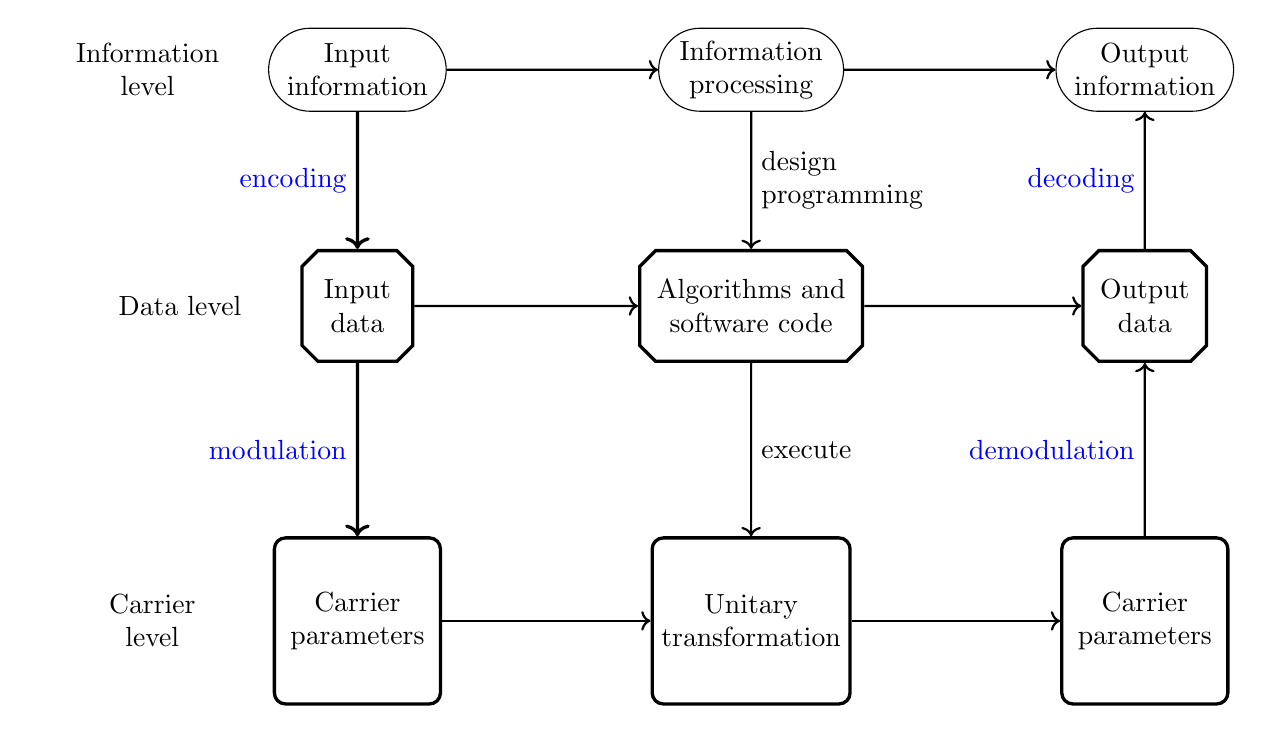
\begin{tikzpicture}[
info/.style={rounded rectangle, draw=black, minimum size=30, align=center},
symbol/.style={chamfered rectangle, draw=black, very thick, minimum size=40, align=center},
carrier/.style={rounded corners, draw=black, very thick, minimum size=60, align=center},
]

% Define a grid using coordinates
\coordinate (grid1) at (0,0);      % Top-left
\coordinate (grid2) at (5,0);      % Top-center
\coordinate (grid3) at (10,0);      % Top-right
\coordinate (grid4) at (0,-3);     % Middle-left
\coordinate (grid5) at (5,-3);     % Middle-center
\coordinate (grid6) at (10,-3);     % Middle-right
\coordinate (grid7) at (0,-7);     % Bottom-left
\coordinate (grid8) at (5,-7);     % Bottom-center
\coordinate (grid9) at (10,-7);     % Bottom-right

% Nodes at grid points
\node[info] (in) at (grid1) {Input\\information};
\node[info] (proc) at (grid2) {Information\\processing};
\node[info] (out) at (grid3) {Output\\information};

\node[symbol] (sym_in) at (grid4) {Input\\data};
\node[symbol] (sym_proc) at (grid5) {Algorithms and\\software code};
\node[symbol] (sym_out) at (grid6) {Output\\data};

\node[carrier] (qubit) at (grid7) {Carrier\\parameters};
\node[carrier] (gate) at (grid8) {Unitary\\transformation};
\node[carrier] (qubit_out) at (grid9) {Carrier\\parameters};

% Draw levels
\draw (in.west) node[text width=80, align=center, anchor=east] {Information\\level};
\draw (sym_in.west) node[text width=80, align=center, anchor=east] {Data level};
\draw (qubit.west) node[text width=80, align=center, anchor=east] {Carrier\\level};

% Draw connecting arrows
\draw[->, thick] (in) to (proc);
\draw[->, thick] (proc) to (out);
\draw[->, very thick] (in) to node[left, color=blue] {encoding} (sym_in);
\draw[->, thick] (sym_in) to (sym_proc);
\draw[->, thick] (sym_proc) to (sym_out);
\draw[->, thick] (proc) to node[right, align=left] {design\\programming} (sym_proc);
\draw[->, thick] (sym_out) to node[left, color=blue] {decoding} (out);
\draw[->, very thick] (sym_in) to node[left, color=blue] {modulation} (qubit);
\draw[->, thick] (qubit) to (gate);
\draw[->, thick] (gate) to (qubit_out);
\draw[->, thick] (sym_proc) to node[right] {execute} (gate);
\draw[->, thick] (qubit_out) to node[left, color=blue] {demodulation} (sym_out);

\end{tikzpicture}
\end{flushleft}
    \caption{Information technology can be viewed on three levels. The terms with blue font are standard communication terms.}
\end{figure}

Converting information from one representation to numbers or data is called encoding. At the data level, Turing invented the hypothetical Turing machine to study and test algorithms. An algorithm is valid only when it can be run and tested on a Turing machine. Computer science studies data structures and algorithms entirely at this level and does not need to relate to the lower level. A bit of datum is always carried by a bit device at the carrier level.

With Shannon's discovery, studies of information technology, including the study of quantum information technology, can concentrate on the number-symbol and the carrier levels without consideration at the abstract information level.

Relating numbers or symbols to carrier wave parameters is one of the focuses of communication theory called modulation. It is also the focus of quantum information. Demodulation is the reverse of modulation in communication systems. However, it is not the case with quantum systems. Read out from qubits encounters a bottleneck imposed by the fact that each qubit has one unit of energy for measurement.

\subsection{Measuring information}
In information theory, Shannon entropy quantifies the amount of information contained in a sequence of symbols or numbers. Its mathematical formulation is similar to the entropy used in statistical physics. But the former concerns only the numbers which are deemed useful. Their meanings are totally different.

For a set of $N$ symbols or codes, the Shannon entropy reaches its maximum value when all symbols are used with equal frequency. This scenario represents the most compact encoding scheme possible. Throughout this book, we assume that the symbols or numbers we work with have uniform usage probabilities, meaning each symbol is equally likely to occur. Under this assumption, the amount of information they can represent is equal to the Shannon entropy, which is $log_2 N$ bits. Consequently, as the number $N$ increases, the amount of information that the symbols or numbers can represent also increases.

\subsection{Errors}
The height of the mercury column in a blood pressure meter is a real number. Apparently, not the entire range of real numbers is useful. Even within the useful range of 0-300mm, a read-out number may be tainted with errors. If we see the mercury column height is 120.5mm, is it accurate? The tilt of the column may produce what's called systematic error. Environmental factors like table vibrations may introduce random errors. Even 120.5mm is accurate, is it more useful to us than 121mm? If not, we may just take it easy and use only integer readings. Using only integers to represent information is called digital information. Using real numbers is called analog information.

AM and FM radios are probably the only analog communication we still use today. When listening to them, once in a while we hear noise, which is random errors. Therefore, random errors are also called noise in communication. Random errors cannot be corrected. Modern communication technologies all use digital information to avoid systematic errors and get around random errors.

In quantum technologies, the numbers carried by qubits are real numbers -- analog technology. But reading out from the qubits to conventional devices is an analog-digital conversion process, and quantization errors, which is a type of systematic error, may appear. Such quantization errors are rooted in quantum measurement and cannot be improved by equipment improvement. How to get around this fundamental limitation of qubit readout is the focal subject of quantum information.


\section{Using waves to carry information}
\subsection{What are waves?}
\begin{figure}[h]\label{String}
%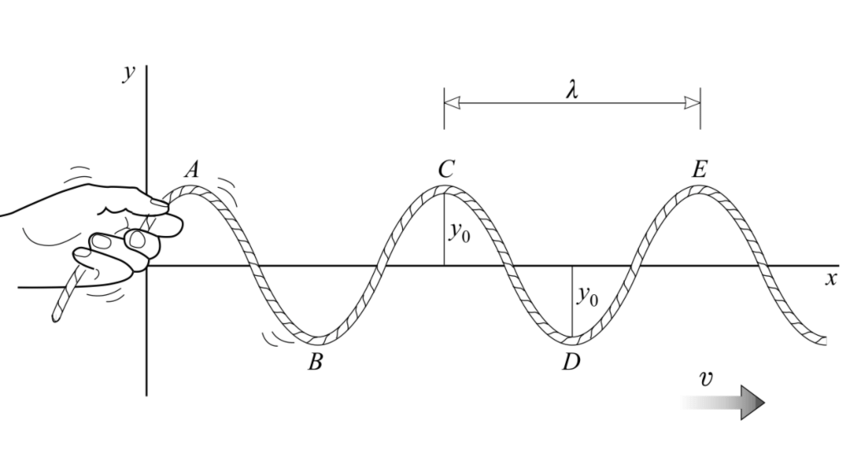
\includegraphics[width=6cm]{pic/wave-in-a-string.png}
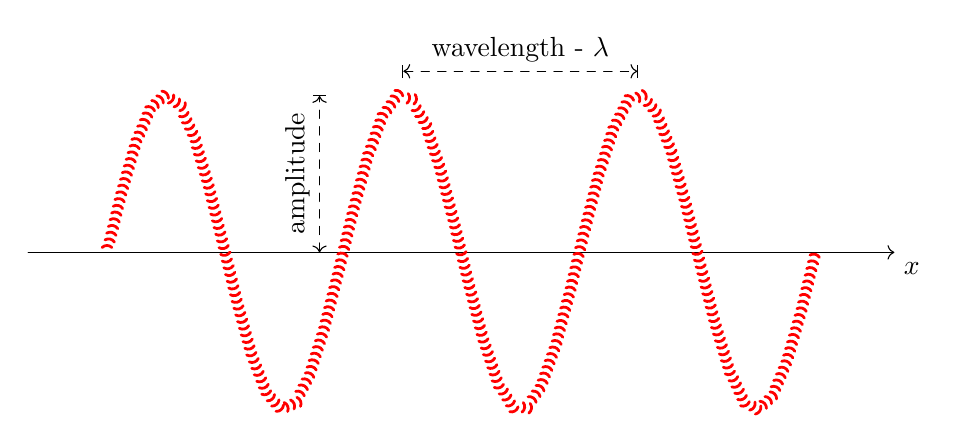
\begin{tikzpicture}[line join=round, line cap=round]

  % draw coordinate
  \draw[->] (-1,0) -- (10,0) node[pos=1.02,below] {$x$};
 % \draw[->] (0, -1) -- (0,2);
  % Rope properties
  \def\length{9}  % Length of the rope
  \def\thickness{1}  % Thickness of the rope
  \def\waveAmplitude{2}  % Amplitude of the wave
  \def\waveLength{3}  % Wavelength
  \def\segments{50}  % Number of segments
  
  % Draw the rope
  \draw[decorate, decoration={waves, segment length=2.5}, line width=\thickness, red]
    (0,0) -- plot[domain=0:\length, samples=\segments]
    (\x, {\waveAmplitude*sin(\x*(360/\waveLength))}) -- (\length,0);

    % label
    %\draw[red, fill] (3.75,2) circle(0.05cm);
    %\draw[red, fill] (6.75,2) circle(0.05cm);
    %\draw[dashed] (2,2) -- (3.75,2);
    \draw[<->|, dashed] (2.7,0) -- (2.7,2) node[pos=0.5, rotate = 90, above] {amplitude};
    \draw[|<->|, dashed] (3.75,2.3) -- (6.75,2.3) node[pos=0.5, above] {wavelength - $\lambda$};

\end{tikzpicture}
\caption{Wave arose from shaking or vibrating a string.}
\end{figure}

When talking about waves, we often visualize ripples in a lake or the surges in oceans and seas. We observe water being pushed up and then pulled down by gravity. If we shake one end of a string, as shown in Fig. \ref{String}, we can observe that each section of the string vibrates, and the vibration propagates from close to far. Vibration\index{vibration} in time and propagation\index{propagation} in space are the fundamental features of all waves. We can use parameters frequency\index{frequency} to characterize how fast the vibration is and amplitude to characterize the height of the vibration. But can we consider the vibration of a guitar string as a wave? Indeed, we can. The reason why we do not perceive propagation is that the propagation gets reflected back and forth by the two fixed ends of the string. Therefore, propagation remains a defining feature of waves, even if their propagation is constrained in spatial dimensions.

Qubits use electromagnetic waves or electron waves. Electromagnetic waves are the vibration of electric and magnetic fields. We are already familiar with radio waves and light waves used in Wi-Fi, cellular, cable, and optical fiber communications, as they are part of our daily lives.

The wave nature of electrons is not obvious because they are trapped to small scales by atomic nuclei. J.J. Thomson discovered how they can be freed from the traps\cite{THOMSON} in a cathode ray tube (CRT). Freed electrons spread to an observable scale and demonstrate all the wave characteristics that physicists had associated with light waves. However, the vibration of an electron wave is not visible like that of a vibrating string or directly measurable like an electromagnetic wave. Physicists do find sufficient evidence of the vibration and have discovered it obeys the Schrödinger wave equation (Dirac equation if Einstein's special relativity is taken into account).

\subsection{Wave parameters}
In Fig. \ref{String}, the height of the rope at any location $x$ along its propagation direction and time $t$ may be described by a wave function $h(x,t)$. The simplest wave function is a sinusoidal function,
\begin{equation}\label{e-hWave}
    h(x,t) = A sin[2\pi (\frac x \lambda - \frac t T) +\phi]
\end{equation}
where $A$ and $\lambda$ are, respectively, the amplitude\index{amplitude} and the wavelength\index{wavelength}, as shown in Fig. \ref{String}. $T$ and $\phi$ are the period\index{period} and phase\index{phase}. Shown but not labeled in Fig. \ref{String} is the polarization\index{polarization}, which refers to the direction of the vibration. The example shown in the figure shows a polarization in the $y$ direction, but it can be in any direction as long as it is perpendicular to the propagation direction. Fig. \ref{Wave} plots the height of the string vibration in the time dimension and is characterized by period\index{period} and phase\index{phase}. All these parameters -- phase, wavelength\index{wavelength}, amplitude\index{amplitude}, period\index{period} and polarization\index{polarization} -- can be used to represent information. Worth noting, that period, wavelength, and frequency are proportional or inversely proportional to each other. Using one is the same as using the others.

\begin{figure}[h]\label{Wave}
\begin{tikzpicture}[scale=1.2]
    \draw[->] (-3.8,0) -- (3.9, 0)  node[pos=1.02,below] {$t$};
    \draw[->] (0,-3.5) -- (0,3.5);
    \draw[dotted, red] (-3.5,0) sin (-2.5,3) cos (-1.5,0) sin (-0.5,-3) cos (0.5,0) sin (1.5,3) cos (2.5,0) sin (3.5,-3);
    \draw[red, fill] (-2.5,3) circle(0.05cm);
    \draw[red, fill] (1.5,3) circle(0.05cm);
    \draw[dashed] (-2.5,0) -- (-2.5,3) node[pos=0.5, rotate = 90, above] {amplitude};
    \draw[dashed] (-2.5,3) -- (1.5,3) node[pos=0.3, above] {period - $T$};
    \draw[red, fill] (0.5,0) circle(0.05cm);
    \draw[dashed] (0.25,-0.1) -- (1,-2) node[below] {phase};
\end{tikzpicture}
\caption{Height of the string vibration in the time domain.}
\end{figure}

\subsection{Using wave parameters to represent data}
In communication, information-carrying waves are called carrier waves or simply carriers\index{carrier}. Choosing wave parameters and mapping them to data is called modulation\index{modulation}. The wave parameters have need to be carefully chosen to avoid noise and errors while maximizing the number of possible parameter points.

Radio broadcasts first used the amplitude of radio waves to represent the volume of one's voice. This is the so-called amplitude modulation (AM). The amplitude is the maximum of the vibrating electric field instead of the maximum height of the vibrating string shown in Fig. \ref{String}. Frequency modulation (FM) was later found less prone to noise than AM in the airways. To this day, we still have both AM and FM on the panels of our radios.

The latest wireless communications, Wi-Fi, 4G and 5G cellphones, all use quadrature amplitude modulation (QAM), which use pairs of amplitude and phase wave parameters. If using each chosen pair of amplitude and phase as a polar coordinate, we can depict the 16-QAM modulation in Fig. \ref{16qam}. It is called a constellation diagram. Each point represents the chosen pair of amplitude and phase. Each is mapped to the 4-bit binary datum below it. A high-end cellphone can support at least 512-QAM modulation, which allows each wave to carry a 9-bit datum.

\begin{figure}%\label{16QAM}
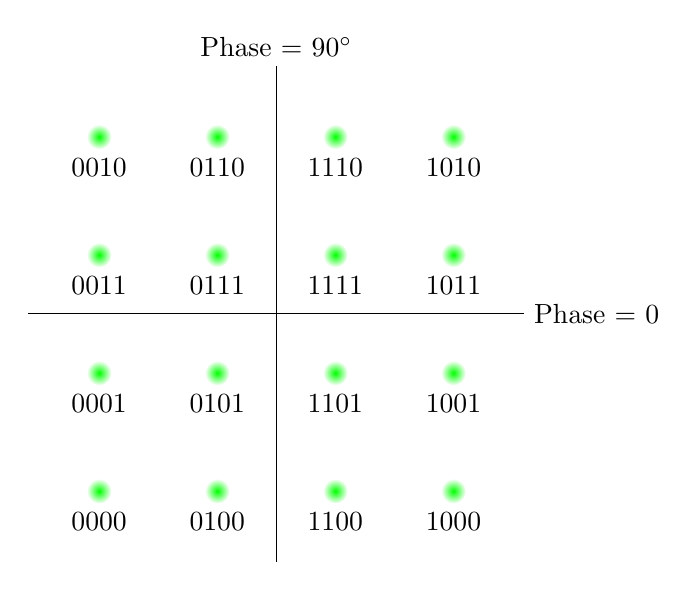
\begin{tikzpicture}[scale=1.5]

% Axis
\draw[] (-2.1,0) -- (2.1,0) node[right] {Phase = 0};
\draw[] (0,-2.1) -- (0,2.1) node[above] {Phase = $90^\circ$};

% Constellation points and labels
\foreach \x/\ix in {-1.5/00, -0.5/01, 0.5/11, 1.5/10} {
    \foreach \y/\iy in {-1.5/00, -0.5/01, 0.5/11, 1.5/10} {
        \shade[shading=radial, inner color=green, outer color=white]  (\x, \y) circle (3pt); % Larger circle with fading edge
        \node[anchor=north] at (\x, \y - 0.1) {\ix\iy}; % Shift labels slightly below
    }
}
\end{tikzpicture}
    \caption{Caption}
\end{figure}

An optical qubit uses a pair polarization and phase parameters to represent a number or datum. Which value pairs of the parameters and which data they map to are determined by how a quantum algorithm uses the qubit. In theory, any real number can be represented. But the mostly used polarizations are 0, 90, 45 and -45 degrees as shown in the constellation diagram of Fig. \ref{qQPSK} and are respectively mapped to 2-bit data 0, 1, 11 and 10. Here phase is assumed to be 0.

\section{The quantum advantage}
\subsection{The quantum theory}
Quantum physics tells us that any wave has its lowest unit -- a quantum\index{quantum} --  when measured by its energy or mass. Plank was the first to toy with the idea. But Einstein was the first to hypothesize this nature of light and called the smallest unit light quantum. Before that, scientists had assumed the energy of light could be dimmed as low as one wishes. What Einstein called a light quantum is today called a photon by physicists. The nature of having the smallest unit is often called the particle nature of matter by physicists nowadays, although calling it the quantum nature is the most accurate.

Einstein's discovery might have something to do with his prior discovery, which equates mass with energy. Until then, all matter was believed to have mass and be composed of elementary particles such as electrons and nuclei. Einstein's revelation that light is also matter may be the precursor of the second revelation of quantum physics: all matter is fundamentally waves.

Bohr was the first to hypothesize electrons being waves. From Einstein and Bohr's hypothesis, the complete theory of quantum physics can be summarized by the particle and wave dual nature of matter:
- all matter is waves and
- each wave's energy or mass is an integer number of its smallest unit.
These two concepts are the essence of quantum physics.

Quantum physics has been successfully applied to the invention and advancement of many modern technologies, including lasers and semiconductors. However, lasers and semiconductor devices involve million to quadrillion photons or electrons. Even the tiniest transistor device in a modern semiconductor chip comprises at least thousands of electrons. However, the advance of making smaller and smaller transistors has gotten us close to the level of working with light or electrons at the individual quantum level.

The idea of using waves at the quantum level is not new. The publication of Deutsch's algorithm\index{Deutsch's algorithm}\cite{1985Deutsch} in 1985 did not garner much attention. But the publication of Shor's algorithm\index{Shor's algorithm} in 1997, which may be considered an extension of Deutsch's, shocked the world with its potential power of factoring large numbers and consequently breaking modern encryption technologies.

The idea of applying quantum technology to secure communication came in 1984 with the publication of BB84 protocol\cite{1997Shor}. The name BB84 is derived from the authors' names -- Bennett and Brassard. The idea is behind the example in introduced in Section-\ref{Sec-example-wifi} and will be discussed in detail in Section-\ref{S-BB84}.

\subsection{The particle nature}
Electrons are called particles for historical reasons. When they are trapped to the small scale of nuclei, they fit the image of point-like particles with negligible sizes and observable locations. This image is certainly wrong if they are freed from the trapping like what J.J. Thomson did in a cathode ray tube. The word "photon" may also carry the annotation of being small in size. The size of a light wave is totally an independent parameter of its energy. The particle nature of matter should be called the quantum nature of matter to avoid misunderstanding. When possible, we shall call a photon a light quantum through the book as Einstein first proposed.

For quantum computing and communication, qubits\index{qubit} -- waves with one quantum of energy or mass in each -- are used to carry information. Appendix-\ref{A-qubit} describes several types of qubits including how they are separated and which wave parameters they use to carry information. The superconductor type is constructed by two superconductors with a thin layer of insulator sandwiched in between. It is not based on any of the fundamental particles, e.g. photons, electrons, and quarks. Physicists have found the energy of the electrons vibrating from one superconductor to another has discrete values. Physicists call such a vibrating wave a pseudo particle. Qubits are easier to make from pseudo particles. But for simplicity, the rest of the book assumes qubits use light or electromagnetic waves.

\subsection{The advantages of analog and digital technologies}
Information technologies have now mostly converted from analog to digital. Not long ago, we used blood pressure meters with columns of mercury. Probably some of us still listen to the AM and FM radios in cars. Analog technologies seem to be something old waiting to die out. The truth is that analog technologies have the advantage of carrying more information. We choose digital technologies only to rid of noise.

Analog technologies represent information as real numbers while digital ones as integers. That is the fundamental difference between the two types of technologies. In the digital world, a real number is rounded off and represented as two integers, the significant and the exponent. The round-off portion is information all lost during the analog-to-digital conversion. The real number $\pi$ may represented in a computer as the integer pair $(31415926, -7)$, which means $31415926*10^{-7}$. The rest $0.5358979...*10^{-7}$ is all lost.

The smallest information-carrying device of a digital computer is a bit, constructed by a pair of transistors. The device's voltage is used to represent information. Two voltage values are used to represent the binary numbers 0 and 1, which are also called a bit number. We could have added more voltage values between the chosen two to increase the numbers being represented. We even could have used all the values, the real numbers, between the chosen two and increased the amount of information represented to infinity -- the case of analog technology. But noise would have obscured the added values and made them useless. Digital technologies gain the advantage of accuracy by sacrificing the amount of information carried and processed. 

Can we take advantage of the information-carrying capacity of analog technologies while avoid the noise problem? Physics tells us that noise is random energy bursts, thermal energy, in particular. But voltage is the potential energy of charged particles and is prone to noise. We should not use any parameter related to energy to represent information. Physics says, waves such as electromagnetic waves have many parameters such as phase and polarization, which are not related to energy.

Yes, that is the idea behind quantum computing:
- separate a wave into discrete elementary waves
- use two real-number parameters of each wave to carry information
- process or manipulate the parameters of all the elementary waves simultaneously to achieve parallel processing.
Why waves and not transistors? Noise! Just about all noise on earth for electronic and optical devices is of some form of thermal energy. If no energy exchange, noise is minimized. Altering a light wave's polarization angle is like changing the direction of a bowling ball's momentum and requires no energy injection. In physicists' words, the transformation of such parameters is unitary. Changing the direction of a bowling ball is a unitary transformation. Changing its speed is not and requires energy exchange.

Another good news is from quantum physics, which says that the energy (or mass) of each of the elementary waves is a fixed value -- a quantum. Adding energy to a wave means adding another elementary wave to it, and the energy increase must be exactly the value of a quantum. This is the so-called quantum nature of waves. It has added the phrase "quantum leap" into our everyday language.

To engineers, the energy parameter of a wave is an integer number and may carry only digital information. Each of the elementary waves that we use to carry analog information is called a quantum bit or qubit for short. The quantum nature determines that qubits are relatively immune to noise because noise injection requires a quantum leap. However, it also sets the limit of qubit readout. It requires energy exchange or transfer to an electronic readout device and is an analog-to-digital data conversion mechanism. Only a binary bit information can be read out from a qubit. This may be why "bit" is in the name of qubit.

The readout limitation narrows the scope that quantum computing has the advantage. The review paper\cite{thermoGoold} authored by Goold etal states "we can write in any real number, but it is only possible
to read one bit out, we cannot copy information ...." But for communication, it can be an advantage for security. The following example shows how.

\section{Application of quantum information}
We are in an information explosion world. In recent years, the rise of AI has further fueled the creation of even more information. ChatGPT’s responses have become quite powerful, yet no one is satisfied — we all expect even more advanced AI. However, the computational power of current computer chips is not sufficient. Major AI companies have already bought out the most powerful GPU chips, driving Nvidia’s stock higher every day. Even with the most powerful GPUs today, training a large language model can take months or even up to a year. So, is there anything more powerful than GPUs? The answer is QPUs—quantum processing units or quantum computers!

Quantum computing is the number one application of quantum information theory. Quantum communication is the second. It has the potential to make encryption key distribution more secure than existing technologies. However, many scientists doubt its importance when comparing the security improvement comparing over the cost.

As a third application, quantum information may be the foundation of studying future-generation devices for integrated circuits. Current chips of integrated circuits are built by transistors as the fundamental devices, whose sizes are now in the nanometers and have met their limits. Any smaller devices may not rely on accumulative physical parameters such as current or voltage to carry information and may need to use individual quantum waves to carry information.

\subsection{The Wi-Fi security problems}\label{Sec-example-wifi}
Electromagnetic waves are used in almost all our communication systems. We see them as light if the wave frequency is in the visible range. The ones used for optical fiber communications are just below the visible frequency range, but we still call them light. The ones used for cable, cellular, and Wi-Fi communications are in the radio frequency range. They are certainly invisible to our naked eyes. But everyone uses them every day and is familiar with them.

Many parameters of electromagnetic waves can be used to carry information. Their parallel exploration ability is another advantage. Before the age of Wi-Fi and cellular communication, we have to find where the network connectors are in the walls to plug in our computers. With Wi-Fi, or computer finds the Wi-Fi router by receiving the radio wave sent in all directions. The radio wave explores all directions in parallel to reach the computer. The broadcasting feature of the communication is a bane, however, for security: the message sent from the Wi-Fi router to my cell phone can be received by an eavesdropping device outside the home. It was once a big concern about using Wi-Fi until encryption was added to the link layer, in the Open System Interconnection (OSI) 7-layer jargon, of the Wi-Fi protocols. Still, the solution has its limit. It would be desirable to have a physical layer solution to fend off eavesdropping.

One naive thinking is to reduce the power of the wave from the router so that only my cell phone can receive the message. But what if the eavesdropper's device is extremely sensitive and can receive the wave at any power level? Indeed, the eavesdropper can still receive the wave until the router lowers the power to contain only a quantum of energy. At this point, the eavesdropper has to capture the entire wave or nothing at all. The wave cannot be split for partial reception. But if the eavesdropper captures the entire wave, I am alerted of the absence of the wave and would suspect the presence of an eavesdropper. This is one of the ideas behind quantum communication and solves the eavesdropping problem halfway. But continuing with the quantum nature of waves, we can add encryption to the solution, for which we will leave the details to Section-\ref{S-BB84}.

\begin{figure}[h]\label{Room-WiFi}
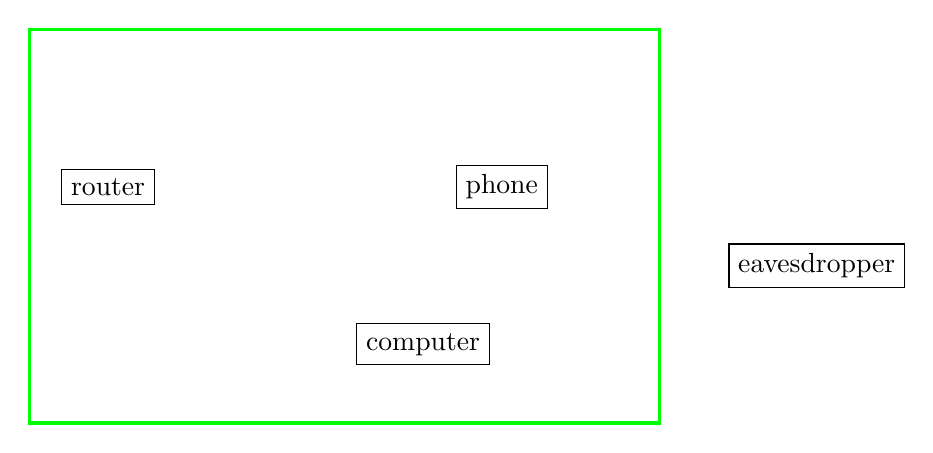
\begin{tikzpicture}
\draw[green, very thick] (0,0) rectangle (8,5);
\draw (1,3) node(router) [rectangle, draw] {router};
\draw (6,3) node(phone) [rectangle, draw] {phone};
\draw (5,1) node(computer) [rectangle, draw] {computer};
\draw (10,2) node(eavesdropper) [rectangle, draw] {eavesdropper};
\end{tikzpicture}
\caption{Wi-Fi}
\end{figure}

\subsection{Constructing a quantum computer}
The core of a quantum computer may use quantum waves to store and process information. However, other components of the computer still uses conventional computer hardware and software. We interact with the computer just like with any other computer. We can even use most of the general-purpose programming languages such as Python to program the quantum computer. Only the portion of a program that needs the power of quantum computing invokes a quantum circuit.

As an example, the Python code below implements Deutsch's algorithm described in Section-\ref{S-Deutsch}.
\begin{lstlisting}
from qiskit import QuantumCircuit, Aer, execute
# Define the quantum circuit with 1 qubit and 0 classical bit
qc = QuantumCircuit(1, 0)
# Apply quantum gates to the qubit
qc.h(0)
qc.x(0)
qc.h(0)
# Measure the qubit and output a 0-or-1 answer
qc.measure([0, 1])
# Draw the circuit
print(qc.draw())
\end{lstlisting}
The code starts by importing the class "QuantumCircuit" from package "qiskit" provided by IBM before applying quantum gates to it. The "measure" gate reads out the computation result from the qubit. 

In the standard von Neumann computer architecture, a register\index{register} is an information memory device; and a gate is an information processing device. A processing unit\index{processing unit} is a circuit comprised of two types of devices. A quantum processing unit also adheres to this von Neumann architecture. Fig. \ref{Circuit} is a quantum circuit diagram\index{quantum circuit diagram} invoked by the above program. Each line in the diagram is a quantum register -- a qubit. Information is represented in analog form. "H" and "CX" gates are drawn as rectangular boxes in the diagram. The gates, applied from left to right according to the sequence in the diagram, transform the wave parameters in the qubits they connect to and thus process the information represented. A double-line is a conventional register -- a bit. The "Measure" gate reads the parameters of the wave in a qubit and outputs the result in digital form to a conventional memory depicted as a double line.

Despite being in Python, a high-level language, the code still calls on registers and gates like code in an assembly language, which programmers worked with 50 years ago. To program, we need the circuit diagram. To design the circuit, we need the protocol or algorithm. This book starts with how information is stored and processed by quantum devices before describing the most popular algorithms and protocols, and their circuit diagrams.

\begin{figure}\label{Circuit}
    \centering
\begin{quantikz}%[slice all, slice style={shorten <=8mm}, slice label style = {yshift=-38mm} ]
    \lstick{qubit 0} & \gate{H} & \gate[2]{CX} & \meter{}  & \cw \rstick{Output bit 0}\\
    \lstick{qubit 1} & \qw      &           & \meter{} & \cw \rstick{Output bit 0}
\end{quantikz}
    \caption{Quantum circuit}
\end{figure}

\chapter{Using waves to carry information}\label{c-modulation}
Computers use digital technologies at the very beginning of their invention. The ideas and theory behind slide rules, and calculators of analog form, are mostly lost in history. Communication systems, on the other hand, have gone through a long period of using analog technologies to mostly digital technologies today. Communication theory is well-developed in the study of information in both analog and digital forms. Further, modern communication systems use electromagnetic waves exclusively as information-carrying media. The wealth of knowledge accumulated in communication theory is most apt for the study of quantum computing and communication. The only addition needed is on the qubit readout mechanism, which will be discussed in the next chapter. This chapter reviews some of the key subjects in communication theory.

\section{Phase modulation}
The phase of a wave reflects its relative time delay in propagation. Changing the phase value can be achieved by adding or subtracting the propagation path of the wave. Usually noted by $\phi$, phase can take up any real number in the range $[0, 2 \pi)$. Using it as real numbers to represent information is an analog modulation. Using selected values to represent information is a digital modulation. All qubits include phase modulation, which is always combined with polarization modulation (or equivalent) to carry information.

\subsection{Graphical depiction and mathematical notation}
In communication textbooks, amplitudes and phases of waves are paired as polar coordinates to plot the modulation points. Such a plot is called a constellation diagram. It gives us the most intuitive understanding of modulations. In phase modulation, the amplitude $A$ is a constant. The modulation points all fall on the circle of radius $A$ as shown in red in Fig. \ref{PM}.

\begin{figure}[h]\label{PM}
\begin{tikzpicture}
    \draw[->] (-3.5,0) -- (3.5, 0);
    \draw[->] (0,-3.5) -- (0,3.5);
    \draw[dotted, red] (0,0) circle(3cm);
    \draw[red, fill] (30:3) circle(0.05cm);
    \draw[dashed] (1,0) arc (0:30:1) node[right, pos=0.6]{$\varphi$ - phase};
    \draw[dashed] (30:0.1) -- (30:2.9) node[pos=0.5, rotate = 30, above] {amplitude};
\end{tikzpicture}
\caption{Phase modulation constellation diagram}
\end{figure}

The polar coordinate $(A, \phi)$ can also be written in Cartesian coordinates as $(A cos\phi, A sin\phi)$ or as a complex number $A e^{i\phi}$. The polar coordinate notation is easier for geographic understanding. The latter two notations are most useful for mathematical derivation.

From the constellation diagram and the Cartesian notation, we see that any modulation point can be regarded as a 2-dimensional vector, which can be decomposed into two vectors, one in the horizontal direction, and the other in the vertical direction. A wave with zero degrees of phase is a vector in the horizontal direction and is called a quadrature wave\index{quadrature wave} by communication engineers. One with $90^\circ$ of phase is a vector in the vertical direction and is called an in-phase wave\index{in-phase wave}.

In practice, any wave can be split into two waves, one in-phase, and the other quadrature whose amplitudes can be determined by the vector decomposition. And, any in-phase wave and quadrature wave can be combined into one whose amplitude and phase can be determined by vector addition of the component waves. or decomposition. Combining two or more waves is called superposition\index{superposition}, a term used by both engineers and physicists. The in-phase and quadrature waves are the vector basis of all waves when represented as vectors in the constellation diagram. We may call them the basis waves.

Worth noting, the selection of the waves with phases of zero and 90 degrees is arbitrary. A wave can be split into any pair of waves whose phases are $90^\circ$ apart. Mathematically, such a pair of waves forms the orthogonal basis of a Hilbert space. To engineers, the advantage of using two orthogonal waves is that they have zero overlap with each other and are maximally distinguishable during demodulation or information readout. This feature will be shown in depth in Section-\ref{Sec-demodulator}.

subsection{Digital modulation}
In the real world, each element in the communication channels and information processing devices can have noise and errors. We must select the modulation points sufficiently apart so that they are not obscured by noise and errors. Therefore, we can only use a finite number of modulation points to which only some integers can be mapped. Digital modulation gains accuracy while sacrificing information-carrying capacity.

All computers use digital technology if we ignore the history of using the slide rule calculators. Even abacuses are digital calculators. Communication systems, however, are slow to convert to digital technology. That is because, for a long time, communication was about transmitting voice -- radio broadcasts and telephones, for which noise and errors could be tolerated. For digital information, modulations often carry different names, e.g., amplitude-shift keying (ASK), frequency-shift keying (FSK), and phase-shift keying, respectively (PSK).

\subsection{Capacity and Hartley's law}
Into a communication channel, in each time slot, an electromagnetic wave is launched with parameters mapping to a symbol. The amount of information transmitted equals the number of possible symbols. However, analog modulation can represent an infinite number of symbols if not considering noise and errors. Its information-carrying capacity may be measured by the bandwidth of the channel.

Digital modulation can carry a countable amount of information to avoid noise and errors. The channel capacity in a digital communication channel is the maximum possible bits per second that can be transmitted. If there are $M$ modulation points, $M$ possible symbols at most can be transmitted per time slot. That is $ln M$ bits of information. If the communication protocol divides each second into $R$ transmission time slots and transmits one wave in each slot, the channel capacity is
\begin{equation}
    C = R ln M.
\end{equation}
This is the so-called Hartley's law. The duration of a wave cannot be shorter than its period. Therefore, $R$ cannot be larger than the frequency of the carrier wave. The frequency is the maximum value of $R$.

\subsection{Quadrature phase-shift keying}
Quadrature phase-shift keying (QPSK) is a digital phase modulation. Its wide use includes several older flavors of Wi-Fi. The later Wi-Fi flavors add more modulation points than the four points in QPSK. QPSK uses modulation points of $\phi being $90 degrees apart from each other. A simple choice is to use $\phi = 0, 90, 180$, and $270$ degrees, which are mapped respectively to 2-bit symbols, 0, 1, 10, and 11 in binary. Fig-\ref{QPSK} is its constellation diagram.

\begin{figure}[h]\label{QPSK}
\begin{tikzpicture}
    \draw[->] (-3.5,0) -- (3.5, 0);
    \draw[->] (0,-3.5) -- (0,3.5);
    \draw[dotted, red] (0,0) circle(3cm);
    \draw[red, fill] (3,0) circle(0.05cm) node[below right] {0};
    \draw[red, fill] (0,3) circle(0.05cm) node[above right] {1};
    \draw[red, fill] (-3,0) circle(0.05cm) node[above left] {10};
    \draw[red, fill] (0,-3) circle(0.05cm) node[below left] {11};
\end{tikzpicture}
%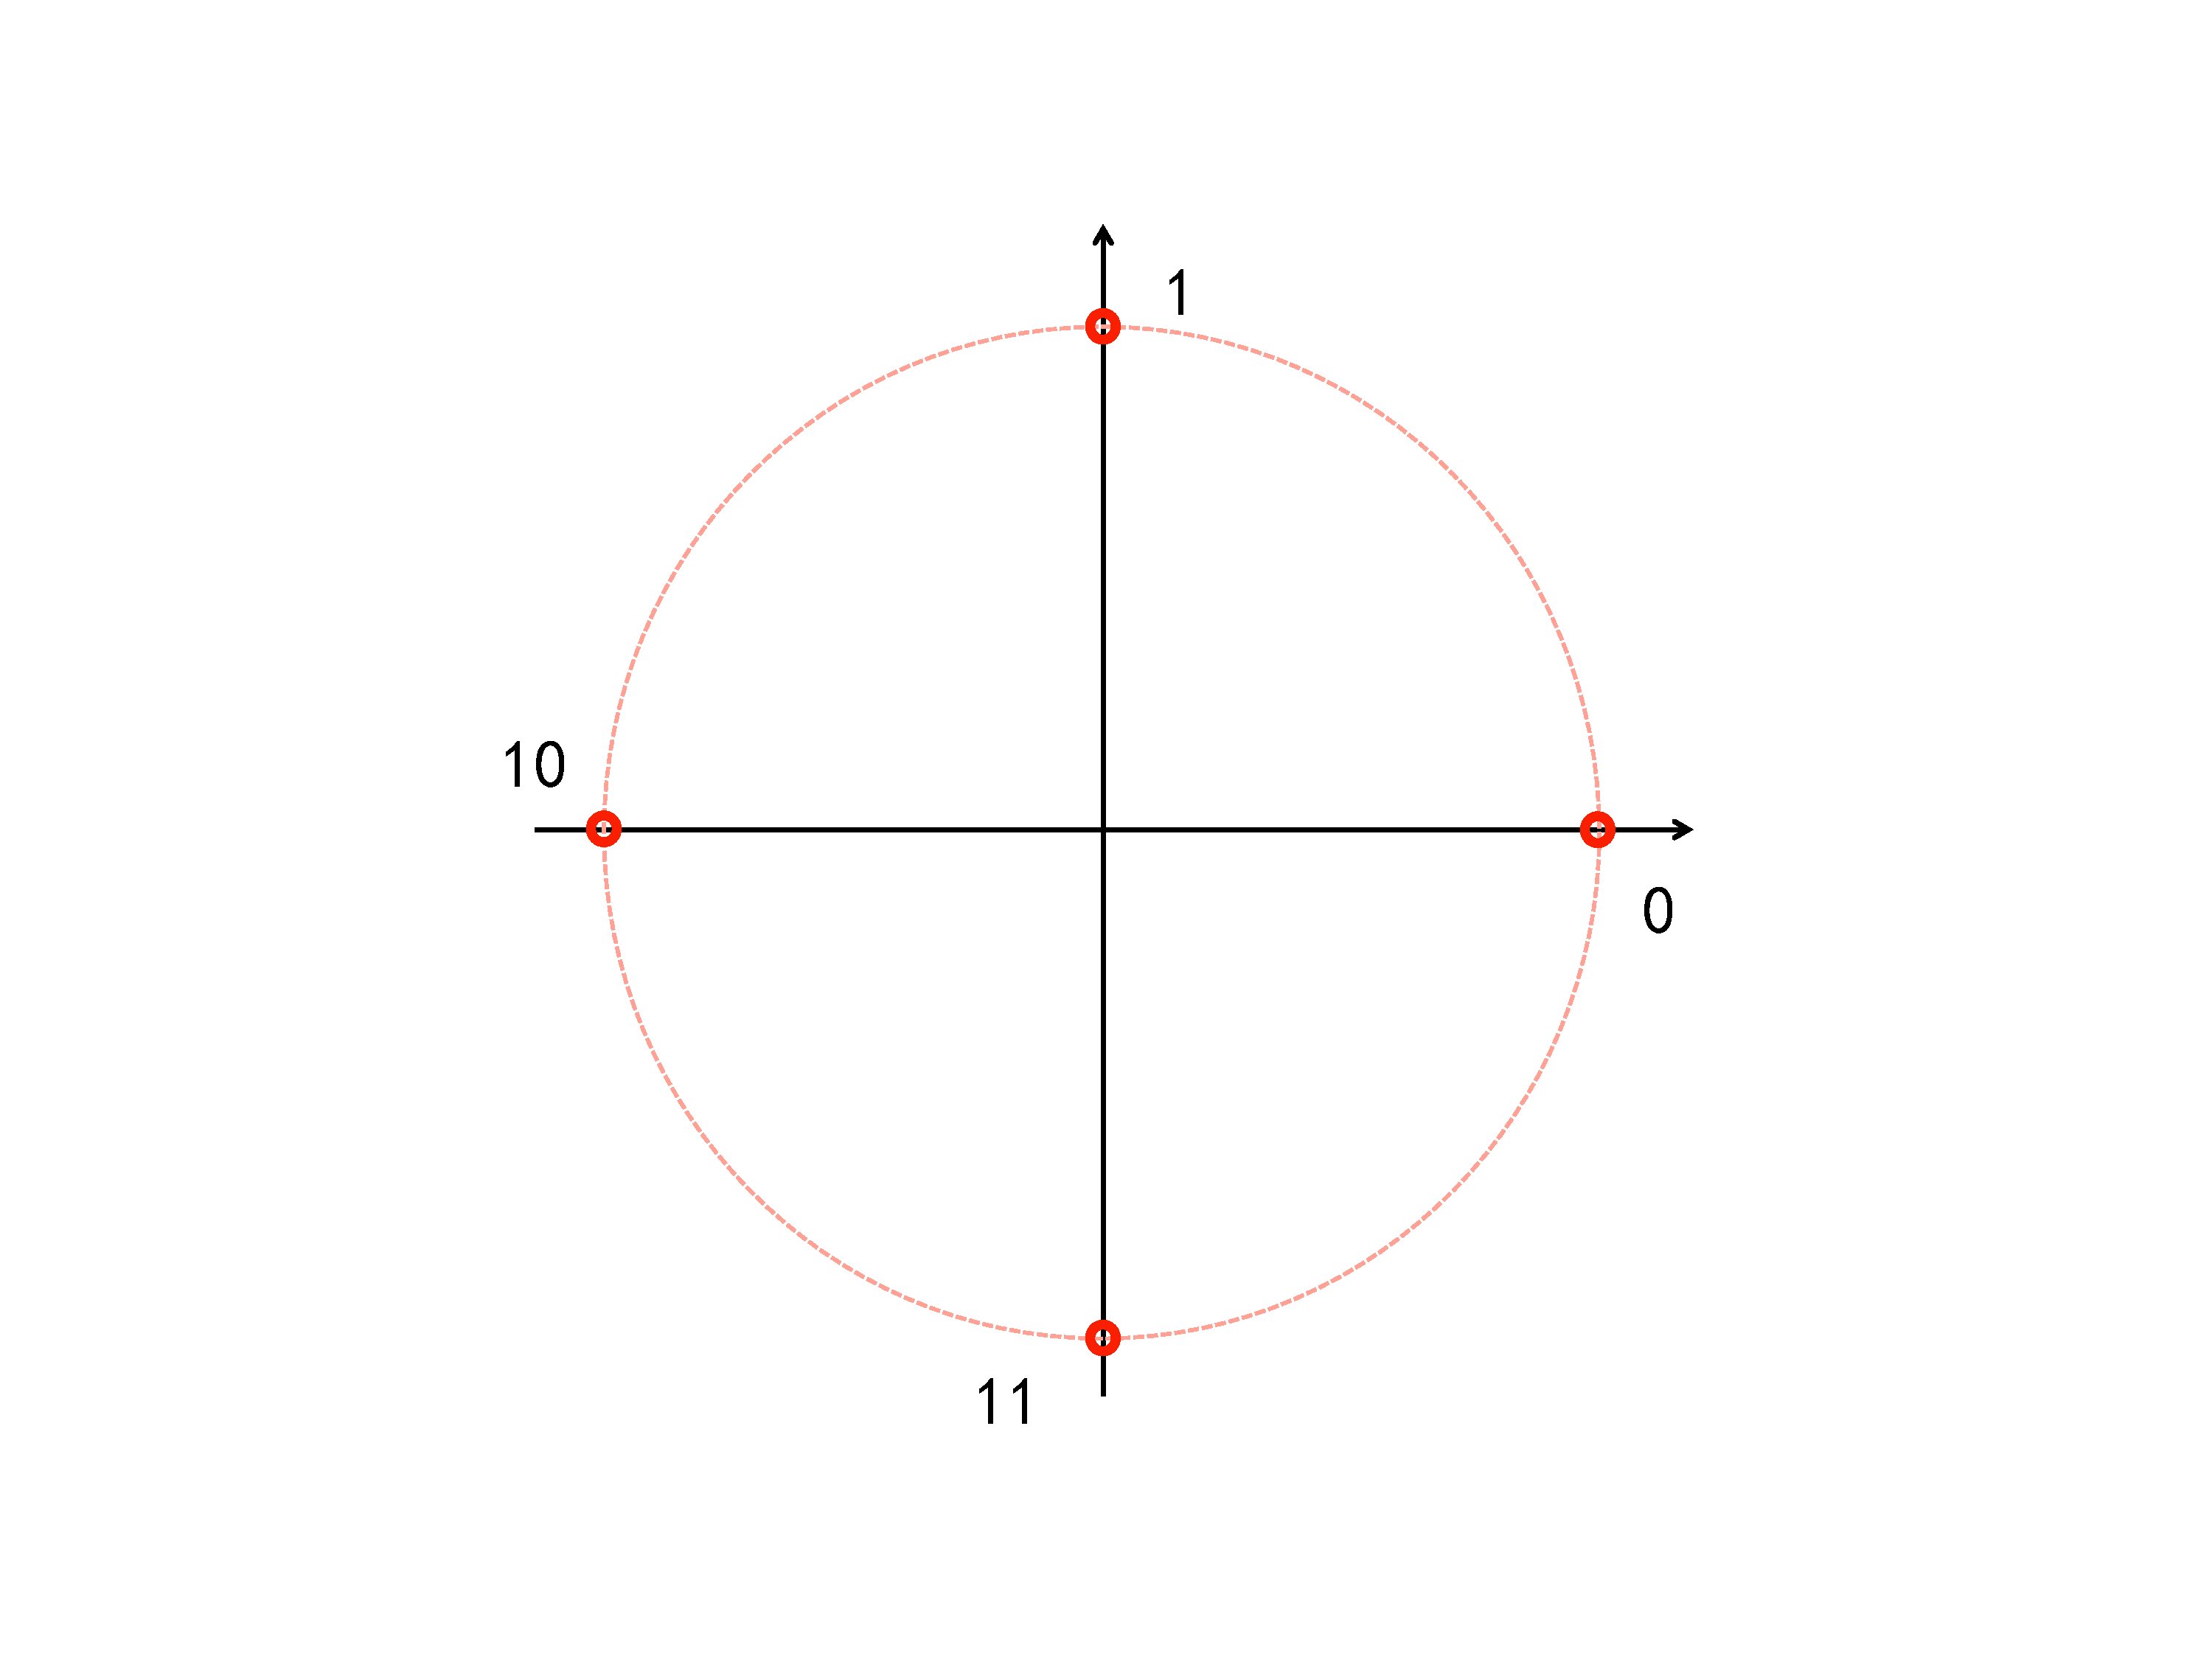
\includegraphics[width=6cm]{pic/4qpsk.pdf}
\caption{QPSK constellation diagram}
\end{figure}

The most popular variation of QPSK is the symmetric QPSK modulation, which is most practical because its modulation and demodulation circuits are the simplest. Its constellation diagram is shown in Fig. \ref{sQPSK}. The modulation points are $\phi = 45, 135, 225$ and $315$ degrees.
\begin{figure}[h]\label{sQPSK}
\begin{tikzpicture}
    \draw[->] (-3.5,0) -- (3.5, 0);
    \draw[->] (0,-3.5) -- (0,3.5);
    \draw[dashed] (2.5,2.5) -- (0, 0);
    \draw[dotted, red] (0,0) circle(3cm);
    \draw[red, fill] (2.12,2.12) circle(0.05cm) node[right] {11};
    \draw[red, fill] (-2.12,2.12) circle(0.05cm) node[above] {01};
    \draw[red, fill] (2.12,-2.12) circle(0.05cm) node[below] {10};
    \draw[red, fill] (-2.12,-2.12) circle(0.05cm) node[left] {00};
    \draw[dashed] (1,0) arc (0:45:1) node[right, pos=0.6]{$\varphi=45\circ$};
\end{tikzpicture}
\caption{Symmetric QPSK constellation diagram}
\end{figure}

\subsection{Modulator and demodulator for symmetric QPSK}\label{Sec-demodulator}
A device that sets or alters a wave's parameter to represent information is called a modulator\index{modulator}. A device that reads out the information carried by a wave is called a demodulator\index{demodulator}. Fig. \ref{modulator} is the circuit block diagram of a symmetric QPSK modulator. Each block in the diagram is a chip or device with well-known functions. The single lines represent wave transmission lines. We may imagine it is the modulator in our Wi-Fi router. The wave output on the right feeds into an antenna to go into the air. The double lines are electronic data lines. A stream of data bits, probably from the Internet, comes in from the left as electrical current or voltage pulses.

The modulator can transmit two bits in each time slot: the odd bit modulates the quadrature wave, and the even bit modulates the in-phase wave. In each branch, an input bit of zero shifts the phase of the wave by $180^\circ$ while the bit of "1" causes no phase shift. The combined wave in the output has a phase of $45, 135, 225$ or $315$ degrees.

\begin{figure}[ht]\label{modulator}%modulator1
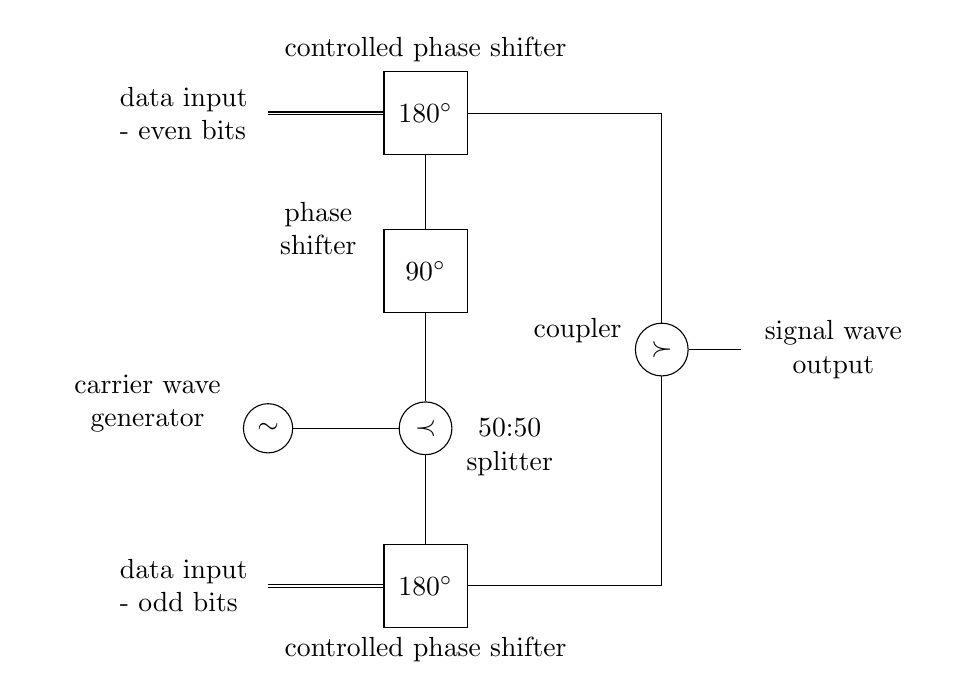
\begin{tikzpicture}
    \path
    (-2,-1) node[circle, draw=black] (lo) {$\sim$}
    (0,-1) node[circle, draw=black] (splitter) {$\prec$}
    (0,1) node[Gate] (p90) {$90^\circ$}
    (0,3) node[Gate] (ta) {$180^\circ$}
    (0,-3) node[Gate] (ba) {$180^\circ$}
    (3,0) node[circle, draw=black] (coupler) {$\succ$}
     (4,0) node[text width=60, align=center, anchor=west] (output) {signal wave output};
    \path (-2,3) node[text width=50, align=left, anchor=east] (even) {data input - even bits}
    (-2,-3) node [text width=50, align=left, anchor=east] (odd) {data input - odd bits};

    \draw (lo.north) node[text width=80, align=center, anchor=east] {carrier wave generator};
    \draw (splitter.south east) node[text width=40, align=center, anchor=west] {50:50 splitter};
    \draw (p90.north west) node[text width=40, align=center, anchor=east] {phase shifter};
    \draw (ta.north) node[anchor=south] {controlled phase shifter};
    \draw (ba.south) node[anchor=north] {controlled phase shifter};
    \draw (coupler.north west) node[text width=40, align=center, anchor=east] {coupler};
    \draw (coupler) -- (output);
    \draw (ba) -- (splitter) -- (p90) -- (ta) -| (coupler) |- (ba);
    \draw (lo) -- (splitter);
    \draw[double] (even) -- (ta);
    \draw[double] (odd) -- (ba);
\end{tikzpicture}
\caption{QPSK modulator circuit}
\end{figure}

The demodulator circuit is basically a reverse of the modulator as shown in Fig. \ref{Demodulator}. The two outputs of the local wave generator have phases at zero and $90^\circ$. Each is mixed with 50\% of the signal wave to produce resonance. The mix of two waves with agreeing phases resonant positively and produces an electric current in the following detector. Two waves with $180^\circ$ phase difference resonant negatively and produce no current. The presence or absence of the current outputs the symbol "1" or "0."

\begin{figure}[h]\label{Demodulator}
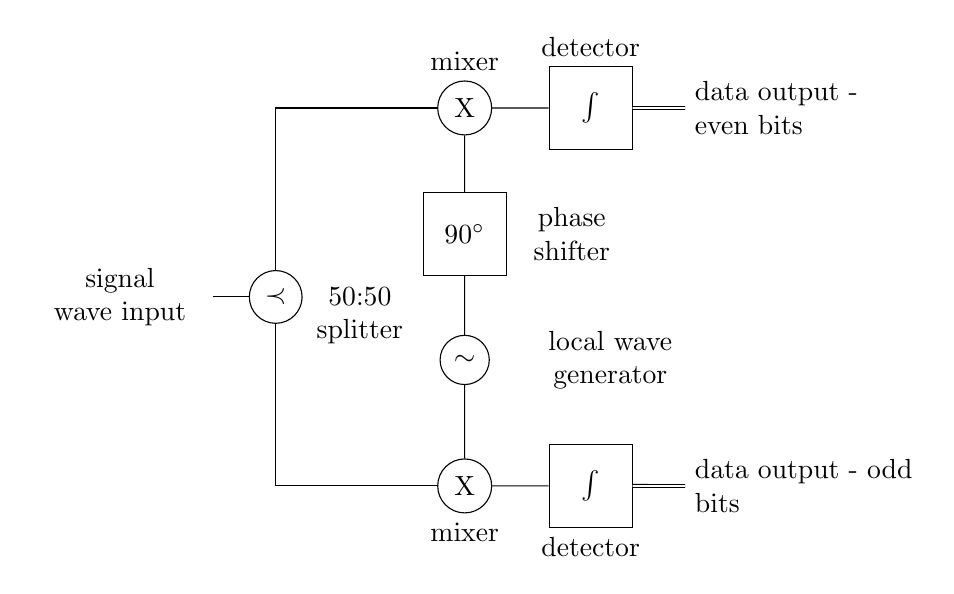
\begin{tikzpicture}[scale=0.8]
    \path
    (0,-1) node[circle, draw=black] (lo) {$\sim$}
    (0,1) node[Gate] (p90) {$90^\circ$}
    (0,3) node[circle, draw=black] (ta) {X}
    (0,-3) node[circle, draw=black] (ba) {X}
    (2,3) node[Gate] (tm) {$\int$}
    (2,-3) node[Gate] (bm) {$\int$}
    (-3,0) node[circle, draw=black] (split) {$\prec$}
     (-4,0) node[text width=60, align=center, anchor=east] (input) {signal wave input};
    \path (3.5,3) node[text width=80, align=left, anchor=west] (even) {data output - even bits}
    (3.5,-3) node [text width=80, align=left, anchor=west] (odd) {data output - odd bits};

    \draw (lo.east) node[text width=80, align=center, anchor=west] {local wave generator};
    \draw (p90.east) node[text width=40, align=center, anchor=west] {phase shifter};
    \draw (tm.north) node[anchor=south] {detector};
    \draw (bm.south) node[anchor=north] {detector};
    \draw (ta.north) node[anchor=south] {mixer};
    \draw (ba.south) node[anchor=north] {mixer};
    \draw (bm) -- (ba) -- (lo) -- (p90) -- (ta) -- (tm);
    \draw[double] (even) -- (tm);
    \draw[double] (odd) -- (bm);

    \draw (ba) -| (split)  |- (ta);
    \draw (split.south east) node[text width=40, align=center, anchor=west] {50:50 splitter};
    \draw (split) -- (input);    
\end{tikzpicture}
    \caption{Symmetric QPSK demodulator.}
\end{figure}

\section{Polarization modulation}
The polarization of an electromagnetic wave is the direction of vibration of its electric field, which is always in the $x-y$ plane if assuming $z$ is the direction of propagation. If the polarization is consistently in one direction, it is called linear polarization and can be characterized by its angle to the $x$ axis $\theta$. The parameter $\theta$ can be used to represent information.

\subsection{Graphical depiction and mathematical notion}
As with phase modulation, a linearly polarized wave can be represented as a vector in the $x-y$ plane or as a point on a circle in a constellation diagram shown in Fig. \ref{PolarM}. The vector's length reflects the wave's amplitude. It can be represented in polar coordinates as $(A, \theta)$, or in Cartesian coordinates as $(A cos\theta, A sin\theta)$.

As with phase, a linearly polarized wave can be separated into two component waves whose polarizations are orthogonal, e.g. one in the horizontal and the other vertical direction. The selection of the $x$ and $y$ axes can be arbitrary as long as they are orthogonal and perpendicular to the propagation direction. Appendix-\ref{A-qubit} describes briefly how a polarization splitter can separate the component waves. Any textbook on optics can be referenced on this subject in detail.

As with phase, the superposition of two waves of horizontal and vertical polarizations is a wave of polarization whose angle $theta$ is determined by the ratio of the two waves: $A_y/A_x = tan\theta$. Mathematically, the two waves are the vector basis of all waves when represented as vectors in the constellation diagram shown in Fig. \ref{PolarM}. Physicists may call them the basis waves.

\begin{figure}[h]\label{PolarM}
\begin{tikzpicture}
    \draw[->] (-3.5,0) -- (3.5, 0);
    \draw[->] (0,-3.5) -- (0,3.5);
%    \draw[dotted, red] (0,0) circle(3cm);
    \draw[dotted, red] (3,0) arc(0:180:3);
    \draw[red, fill] (30:3) circle(0.05cm);
    \draw[dashed] (1,0) arc (0:30:1) node[right, pos=0.6]{$\theta$};
    \draw[dashed] (30:0.1) -- (30:2.9) node[pos=0.5, rotate = 30, above] {amplitude};
\end{tikzpicture}
\caption{Polarization modulation constellation diagram}
\end{figure}

\subsection{Elliptical polarization}\label{s-elliptic}
In the above discussion, we see that the superposition of two orthogonal linearly polarized waves is another wave of linear polarization. But that is under the assumption that the two waves are of equal phase. What happens if the two waves have different phases? That is to say, the wave with polarization in the $x$ direction is $A cos\theta e^{i\phi_x}$, and the one in the $y$ direction is $A sin\theta e^{i\phi_y}$. Their superposition is a wave we call elliptical polarization because the electrical field (a vector) of such a wave changes throughout the vibration period in an elliptic pattern. The propagation of the electric field, on the other hand, is a helical pattern as shown in Fig-\ref{CircularP}.

Linear polarization is a special case of elliptical polarization when $\phi = \phi_y-\phi_x$ is zero or $180^\circ$. Another special case is circular polarization for which $\phi$ is $90^\circ$ or $270^\circ$.

\begin{figure}[h]\label{CircularP}
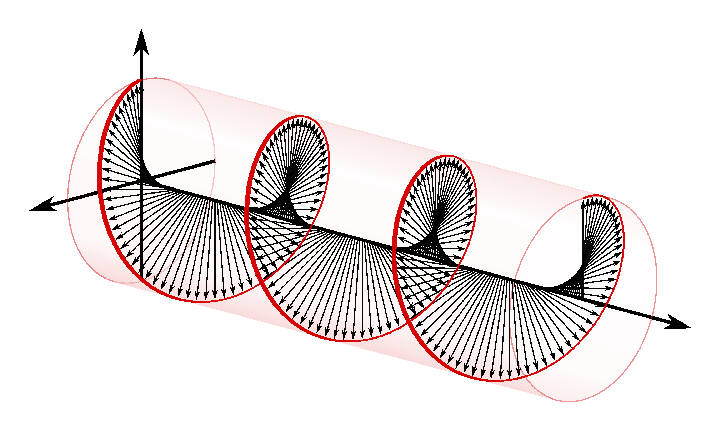
\includegraphics[width=10cm]{pic/CircularPolarization.eps}
\caption{The vector of the vibration of the electric field}
\end{figure}

Elliptical polarization modulation uses the three tuples $(A, \theta, \phi_x)$ to represent information. It has only been proposed for use in space-space communication by researchers\cite{Circular-Wang} without real deployment. But for quantum communication and computing, elliptical polarization modulation and the equivalent are used exclusively. The subject will be discussed in detail in the next chapter.

\subsection{Dual-polarization quadrature phase shift keying}
Modern optical fiber and free space communication use a digital form of elliptical polarization dual-polarization quadrature phase shift keying\index{dual-polarization quadrature phase shift keying} (DP-QPSK\index{DP-QPSK}), polarization modulation\index{polarization modulation} is not used alone but rather in combination with phase modulation. This is mostly used in particular. Optical fiber communication is the backbone of all our daily communication. Free-space communication, on the other hand, is mostly used in earth-satellite and satellite-satellite communication.


Assuming one wave has polarization of $\theta=45^circ$ and the other of $135^\circ$, Fig. \ref{PolarM} is a 3-D constellation depiction showing the 8 modulation points -- call on a 3-D sphere. Phase or polarization modulation alone can use a 2-D constellation diagram like Fig. \ref{PM} or Fig. \ref{PolarM} to depict. Graphically showing a modulation combining both parameters needs to use the polar coordinates $(A, \theta, \psi)$. It shows that the eight digital modulation points all lie on a sphere of radius that equals the amplitude $A$. Here $\theta$ is between $0-180\circ$ because the wave with $(A, \theta+180^\circ, \phi$ is the same as $(A, \theta, \phi+180^\circ$.

%\node [constellation_cir] at (0,0) {};
\begin{figure}[h]\label{DP-QPSK}
\tdplotsetmaincoords{75}{110}
\pgfmathsetmacro{\h}{3.53}
\pgfmathsetmacro{\hn}{-3.53}
\pgfmathsetmacro{\r}{5}
\pgfmathsetmacro{\rn}{-5}
\pgfmathsetmacro{\ang}{105}
\begin{tikzpicture}[tdplot_main_coords]
\tdplotsetcoord{P1}{\r}{45}{45}
\tdplotsetcoord{P2}{\r}{-45}{45}
\tdplotsetcoord{P3}{\r}{45}{-45}
\tdplotsetcoord{P4}{\r}{-45}{-45}

\tdplotsetcoord{P5}{\r}{135}{45}
\tdplotsetcoord{P6}{\r}{-135}{45}
\tdplotsetcoord{P7}{\r}{135}{-45}
\tdplotsetcoord{P8}{\r}{-135}{-45}

\shade[ball color=gray, tdplot_screen_coords, opacity=0.10] (0,0,0) circle [radius=\r];

% xy plane
\tdplotdrawarc[gray]{(0,0,0)}{5}{-75}{\ang}{};
\tdplotdrawarc[dashed, gray]{(0,0,0)}{\r}{\ang}{285}{};
% yz plane
\tdplotsetthetaplanecoords{90}
\tdplotdrawarc[tdplot_rotated_coords, gray!70]{(0,0,0)}{\r}{-38}{157}{};
\tdplotdrawarc[tdplot_rotated_coords,dashed, gray]{(0,0,0)}{\r}{150}{335}{};

% xyz axes
\draw[dashed, gray!50] (\rn,0,0) -- (0,0,0); \draw[gray!50] (0,0,0) -- (\r,0,0);
\draw[gray!55] (0,\rn,0) -- (0,\r,0);
\draw[gray!60] (0,0,\rn) -- (0,0,\r);
\draw[thick, -Stealth] (\r,0,0) -- (9,0,0) node[black, left] {$x$};
\draw[thick, -Stealth] (0,\r,0) -- (0,7,0) node[black, right] {$y$};
\draw[thick, -Stealth] (0,0,\r) -- (0,0,7) node[black, left] {$z$};

% points
\fill[red] (P1) circle (0.1); \fill[red!50] (P2) circle (0.1);
\fill[red] (P3) circle (0.1); \fill[red!50] (P4) circle (0.1);
\fill[red] (P5) circle (0.1); \fill[red!50] (P6) circle (0.1);
\fill[red] (P7) circle (0.1); \fill[red!50] (P8) circle (0.1);
\node[above] at (P1) {$(\frac \pi 4, \frac \pi 4)$};
\node[below] at (P2) {$(\frac \pi 4, \frac {5\pi} 4)$};
\node[above right] at (P4) {$(\frac \pi 4, \frac {3\pi} 4)$};
\node[below left] at (P3) {$(\frac \pi 4, \frac {7\pi} 4)$};
\node[above] at (P5) {$(\frac {3\pi} 4, \frac \pi 4)$};
\node[above] at (P6) {$(\frac {3\pi} 4, \frac {5\pi} 4)$};
\node[above right] at (P8) {$(\frac {3\pi} 4, \frac {3\pi} 4)$};
\node[below left] at (P7) {$(\frac {3\pi} 4, \frac {7\pi} 4$};

\draw[dashed, red!70] (0,0,0) -- (2.5, 2.5, 0) -- (P1) -- cycle;
\draw[dashed, red!30] (0,0,\h) circle (\h);
\draw[dashed, red!30] (0,0,\hn) circle (\h);

\tdplotsetthetaplanecoords{45}
\tdplotdrawarc[tdplot_rotated_coords, -Latex]{(0,0,0)}{2}{0}{45}{anchor=north east}{$\theta$}

\draw [thick, -Latex, canvas is xy plane at z=0] (2,0) arc [start angle=0, end angle=45, radius=2];
\node at (2,0.5,-0.3) {$\phi$};

\end{tikzpicture}
\caption{Modulation points of DP-QPSK}
\end{figure}

\subsection{DP-QPSK modulator and demodulator}
Fig. \ref{Modulator-DP-QPSK} shows a DP-QPSK modulator. It uses two waves of orthogonal linear polarization from the same source, and each is modulated with 2 bits using QPSK. The two waves are then combined to feed into one communication medium such as an optical fiber. A DP-QPSK modulator circuit diagram is shown in Fig. \ref{Modulator-DP-QPSK}. A demodulator is shown in Fig. \ref{Demodulator-DP-QPSK}.

\begin{figure}\label{Modulator-DP-QPSK}
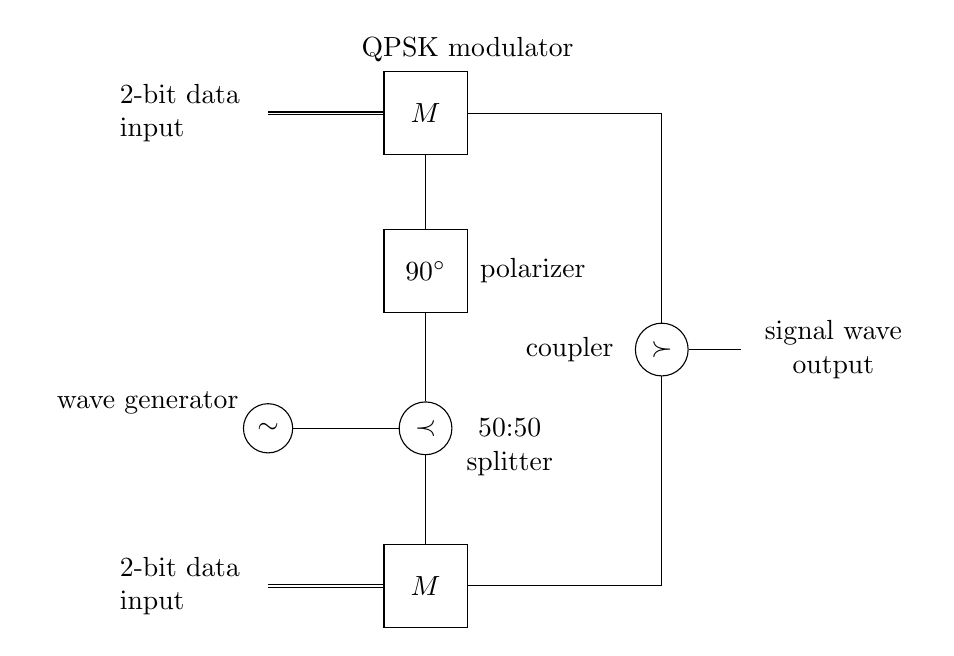
\begin{tikzpicture}
    \path
    (-2,-1) node[circle, draw=black] (lo) {$\sim$}
    (0,-1) node[circle, draw=black] (splitter) {$\prec$}
    (0,1) node[Gate] (p90) {$90^\circ$}
    (0,3) node[Gate] (ta) {$M$}
    (0,-3) node[Gate] (ba) {$M$}
    (3,0) node[circle, draw=black] (coupler) {$\succ$}
     (4,0) node[text width=60, align=center, anchor=west] (output) {signal wave output};
    \path (-2,3) node[text width=50, align=left, anchor=east] (even) {2-bit data input}
    (-2,-3) node [text width=50, align=left, anchor=east] (odd) {2-bit data input};

    \draw (lo.north) node[text width=80, align=center, anchor=east] {wave generator};
    \draw (splitter.south east) node[text width=40, align=center, anchor=west] {50:50 splitter};
    \draw (p90.east) node[text width=40, align=center, anchor=west] {polarizer};
    \draw (ta.north east) node[anchor=south] {QPSK modulator};
    \draw (coupler.west) node[text width=40, align=center, anchor=east] {coupler};
    \draw (coupler) -- (output);
    \draw (ba) -- (splitter) -- (p90) -- (ta) -| (coupler) |- (ba);
    \draw (lo) -- (splitter);
    \draw[double] (even) -- (ta);
    \draw[double] (odd) -- (ba);
\end{tikzpicture}
    \caption{DP-QPSK modulator circuit block diagram}
\end{figure}

\begin{figure}\label{Demodulator-DP-QPSK}
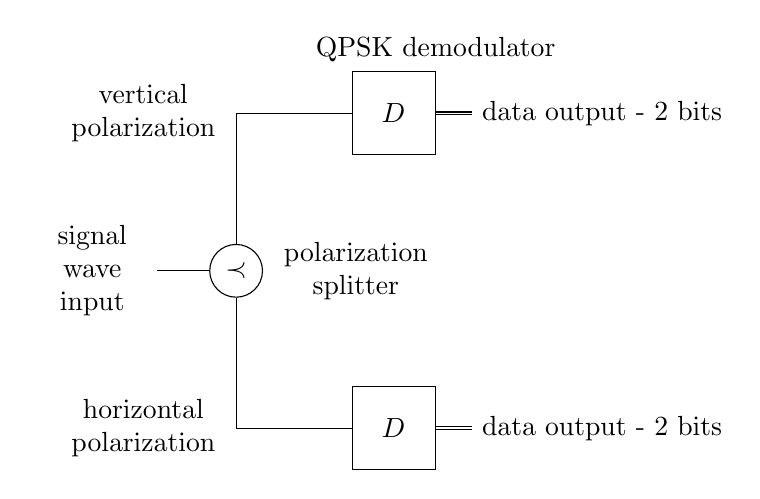
\begin{tikzpicture}[scale=1]
    \path
    (-3,0) node[text width=40, align=center, anchor=east] (input) {signal wave input}
    (-2,0) node[circle, draw=black] (split) {$\prec$}
    (0,2) node[Gate] (tsp) {$D$}
    (0,-2) node[Gate] (bsp) {$D$};
     
    \path 
    (-2,2) node [text width=60, align=center, anchor=east] (V) {vertical polarization}
    (-2,-2) node [text width=60, align=center, anchor=east] (H) {horizontal polarization}
    (1,2) node [anchor=west] (bit01) {data output - 2 bits}
    (1,-2) node [anchor=west] (bit00) {data output - 2 bits};

    \draw[double] (tsp) -- (bit01);
    \draw[double] (bsp) -- (bit00);
    
    \draw (input) -- (split) |- (tsp);
    \draw (split) |- (bsp);
    \draw (split.east) node[text width=60, align=center, anchor=west] {polarization splitter};
    \draw (tsp.north east) node[anchor=south] {QPSK demodulator};
\end{tikzpicture}
    \caption{DP-QPSK demodulator}
\end{figure}

\chapter{Qubit modulation}\label{c-qinfo}
In the previous chapter, we studied how information can be represented or carried by waves using different modulation schemes. All the modulation schemes, if not involving amplitude modulation, can be used by qubits. Amplitude modulation is excluded because each qubit has only one quantum of energy and its amplitude is fixed and cannot be used to represent different information values. For a qubit, we can assume the amplitude $A=1$.

As introduced in Section-\ref{s-elliptic}, the optical qubits used in quantum communication experiments all adopt the elliptical polarization modulation -- using the polarization angle $\theta$ and the relative phase $\phi$ to carry information. There are many different physical constructs of qubits for quantum computing. Appendix \ref{A-qubit} describes some of them. Instead of polarization, they may use parameters such as frequency, modal, or electron spin. But they are all equivalent to using an angle $\theta$ in combination with the relative phase $\phi$ to represent information. Therefore, we carry out the rest of the discussion as though all qubits use elliptical polarization modulation.

Using two real numbers $\theta$ and $\phi$ to carry information, qubit modulation is analog. However, at the readout, from all the possible real values of the qubit's wave parameters, the demodulator can only output two possible electronic values for reasons we shall explain. Therefore, a demodulator may lead to information loss. And we need to carefully design computation algorithms so that the resulting modulation points may be read out without loss. For communication, on the other hand, we may take advantage of unreadable modulations to conceal or encrypt information -- one of the ideas behind the BB84 protocol described in this chapter.

\section{Modulation and demodulation}\label{S-qModulation}
Modulating a qubit is no different from that described in the previous chapter. Fig. \ref{Modulator-qubit} shows an example modulation circuit. The top one is the conventional circuit block diagram. The polarizer changes the polarization angle $\theta$ for a $\Delta \theta$ amount whose value may be a constant or a variable controlled by a conventional data input or the parameters of other qubits. It shows up in the quantum circuit version in the diagram below as a polarization-altering gate. The phase shifter along with the polarization splitter and coupler in the top diagram form a phase $\phi$ altering gate in the quantum circuit version below. Again, the amount of phase shift may be a constant or a controlled variable. 

\begin{figure}\label{Modulator-qubit}
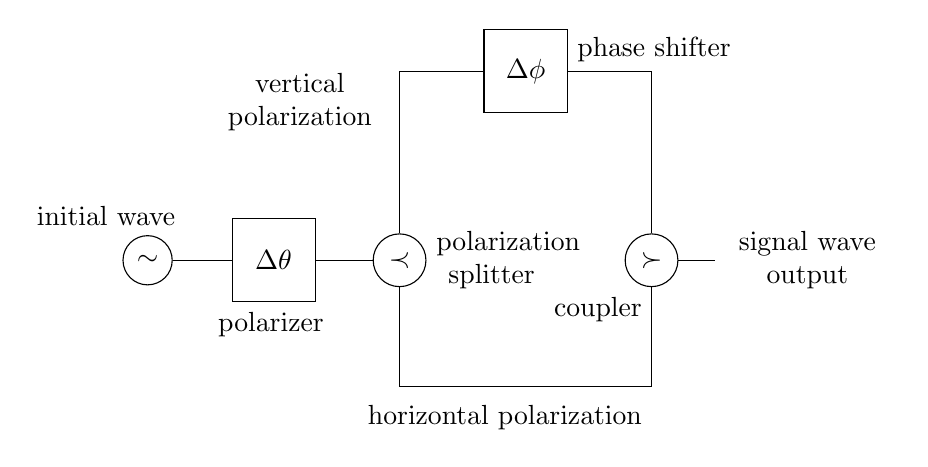
\begin{tikzpicture}[scale=0.8]
    \path
    (-4,0) node[circle, draw=black] (lo) {$\sim$}
    (-2,0) node[Gate] (p90) {$\Delta \theta$}
    (0,0) node[circle, draw=black] (splitter) {$\prec$}
    coordinate[] (H) at (0,-2)
    (2,3) node[Gate] (ta) {$\Delta \phi$}
    (4,0) node[circle, draw=black] (coupler) {$\succ$}
     (5,0) node[text width=60, align=center, anchor=west] (output) {signal wave output};

    \draw (lo.north) node[text width=80, align=left, anchor=south] {initial wave};
    \draw (p90.south) node[text width=40, anchor=north] {polarizer};
    \draw (splitter.east) node[text width=40, align=center, anchor=west] {polarization splitter};

    \draw (ta.east) node[anchor=south west] {phase shifter};
    \draw (coupler.south) node[text width=40, align=right, anchor=north east] {coupler};
    \draw (output) -- (coupler) |- (ta) -| (splitter)
    node[above=2.5, text width=65, align=center, anchor=north east] {vertical polarization};
    \draw (lo) -- (p90) -- (splitter) -- (H) -| (coupler)
    node[below=2, anchor=east] {horizontal polarization};
\end{tikzpicture}
    \caption{Modulation circuit block diagram}

\begin{quantikz}
    \lstick{initial qubit} & \gate{\Delta \theta} & \gate{\Delta \phi} & \qw \rstick{output wave}
\end{quantikz}
    \caption{Quantum circuit diagram}
\end{figure}

\subsection{Demodulation and the readout limitation}
Demodulation is reading out the information from a wave. Physicists call it measurement. It involves energy transfer from a qubit to an electronic device, which is shown in the polarization demodulator circuit block diagram as a detector in Fig. \ref{Demodulator-qubit}. The circuitry is the same for a qubit and a conventional signal wave. For either one, the polarization splitter splits the wave into horizontal and vertical polarization components to resonate with the electrons in the detectors. To demodulate a conventional signal wave, the electric currents generated in the detectors should be proportional to $cos^2\theta$ and $sin^2\theta$ respectively. Therefore, the parameter $\theta$ can be obtained from the ratio of the currents from the two detectors.

The relative phase parameter in a qubit may carry information. But the demodulator does not contain the phase demodulators as the one for DP-QPSK shown in Fig. \ref{Demodulator-DP-QPSK} has because adding them requires adding two more (entangled) qubits as local reference waves and is impractical to have. Therefore phases of the wave components are not measured. And whatever information carried in the phases is lost.

The mechanism of demodulating a qubit is the same as for a conventional wave. But the outcome is different: only one of the detectors may have an electric current and never both. It appears that $\theta$ is either 0 or $\pi/2$ and never in between. Therefore, the readout or decoding of the qubit is limited to only "0" or "1" and nothing in between. That is because there is only one quantum of energy in the qubit, and only one lucky electron in one of the detectors gets a chance to resonate and induce a current. The chance or probability of luck is proportional to $cos^2\theta$ or $sin^2\theta$ depending on which detector it is in.

The phenomenon is very much like tossing a coin into the air, it always collapses to one of the two orientations although it may be in all different orientations in the air. Heisenberg calls the phenomenon wave-function collapse. This kind of phenomenon appears in all quantum measurements and is very puzzling or counterintuitive to physicists because they associate probability with noise and indeterministic. But to engineers, qubit readout is an analog-digital data conversion mechanism -- energy is a discrete number, and rounding off real numbers to integers is nothing strange or counterintuitive.

The qubit readout limitation puts a bound to the power of quantum computing. If at the end of a computation a qubit results in a $\theta$ value of neither 0 nor $\pi/2$, the result cannot be decoded accurately and is useless. We have to design the computation algorithm carefully, including choosing the modulation points at input carefully, so that the qubit results in a $\theta$ value of either 0 or $\pi /2$. The limitation puts a bound to usefulness of quantum computing because the data outcome is limited to one bit per qubit. It also makes designing algorithms hard or challenging. The example Deutsch's algorithm discussed in a later section in this chapter may shed some light on what an algorithm takes to work.

Quantum communication, however, can take advantage of the limitation to make qubits unreadable to eavesdroppers. We will describe how BB84 protocol achieves this in Section-\ref{S-BB84}. Quantum circuit diagrams are good ways to explain an algorithm or protocol. In a diagram, e.g. the bottom half of Fig. \ref{Demodulator-qubit}, a demodulator is shown as a measurement gate or a metering gate. It is called a quantum gate. However, it cannot be expressed as a unitary matrix and is not on the same footing as the other quantum gates.

\begin{figure}\label{Demodulator-qubit}
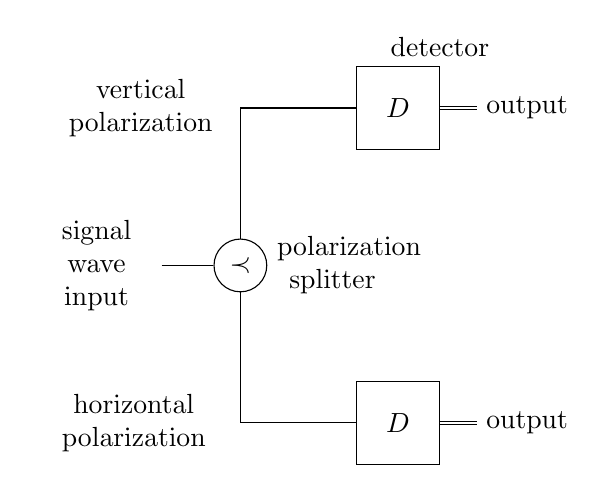
\begin{tikzpicture}
    \path
    (-3,0) node[text width=40, align=center, anchor=east] (input) {signal wave input}
    (-2,0) node[circle, draw=black] (split) {$\prec$}
    (0,2) node[Gate] (tsp) {$D$}
    (0,-2) node[Gate] (bsp) {$D$};
     
    \path 
    (-2,2) node [text width=65, align=center, anchor=east] (V) {vertical polarization}
    (-2,-2) node [text width=70, align=center, anchor=east] (H) {horizontal polarization}
    (1,2) node [anchor=west] (bit01) {output}
    (1,-2) node [anchor=west] (bit00) {output};

    \draw[double] (tsp) -- (bit01);
    \draw[double] (bsp) -- (bit00);
    
    \draw (input) -- (split) |- (tsp);
    \draw (split) |- (bsp);
    \draw (split.east) node[text width=40, align=center, anchor=west] {polarization splitter};
    \draw (tsp.north east) node[anchor=south] {detector};
\end{tikzpicture}
    \caption{Qubit demodulation circuit block diagram}

\begin{quantikz}
    \lstick{input qubit} \qw & \meter{}  & \cw \rstick{output bit}
\end{quantikz}
    \caption{Qubit readout quantum circuit diagram}
\end{figure}

\section{Mathematical notation and graphic depiction}
Continuing from what we learn in previous chapter, an elliptically polarized wave can be noted in the spherical polar coordinates $(A, \theta, \phi_x)$, where $\psi$ is the relative phase, or by a Cartesian coordinate like tensor of complex numbers $(A cos\theta e^{i\phi_x}, A sin\theta e^{i\phi_y})$. The tensor can be written as $(x_0, x_1)$ in general subjected to the condition $|x_0|^2 + |x_1|^2 = 1$ and the assumption $A=1$ for qubits. We may call the complex number pair notation $(x_0, x_1)$ tensor notation. It is convenient when studying a quantum gate, which transforms a qubit from one modulation point to another. For example, if the qubit is transformed to the modulation point $(x'_0, x'_1)$, we can write the transformation as a matrix multiplying the transposed tensor of the original coordinate:
\begin{equation}
    \begin{pmatrix}
    x'_0 \\
    x'_1
\end{pmatrix}
=
    \begin{pmatrix}
    t_{0,0} & t_{0,1} \\
    t_{1,0} & t_{1,1} 
\end{pmatrix}
    \begin{pmatrix}
    x_0 \\
    x_1
\end{pmatrix}.
\end{equation}
Here, the matrix
\begin{equation}\label{e-T}
T
=
    \begin{pmatrix}
    t_{0,0} & t_{0,1} \\
    t_{1,0} & t_{1,1} 
\end{pmatrix}
\end{equation}
is the transformation matrix representing the quantum gate. All matrices transforming a qubit from one modulation point to another are unitary, which means the complex matrix $T^*$ is the inverse of $T$.

\subsection{Dirac ket notation}
Physicists favor what is called the ket notation, which is a vector notation. The unit vectors $\hat x_0$ and $\hat x_1$ are written as $\keta{0}$ and $\keta{1}$. Therefore, a modulation point can be written as $e^{i \phi_0}cos{\theta} \keta{0} + e^{i \phi+1} sin{\theta} \keta{1}$ or $x_0 \keta{0} + x_1 \keta{1}$. Here, the "$+$" is mathematically a vector addition. Physicists interpret the "$+$" as superposition -- mixing or addition of two waves.

The ket notation provides physicists with a brief notation along with associated physical mechanisms. In the ket notation, the transformation of a quantum gate is written as an abstract operator symbol. Therefore, the ket notation is usually used in theoretical derivation while the vector notation is used when numerical calculation is needed.

\subsection{Graphical depiction}
The information carried by a wave in a qubit is represented in the polarization angle $\theta$ and the relative phase $\phi = \phi_1 - \phi_0$ and thus can be described by the pair of real numbers $(\theta, \phi)$. If plotting all the modulation points in spherical polar coordinates, they take up a hemisphere shown in Fig. \ref{bloch-Elliptical} with $A=1$. It is a hemisphere because $\phi$ is a phase difference and the points with $\theta > \pi /2$ duplicate those with $\theta < \pi /2)$ with the reversed $\phi$ value.

The hemisphere is equivalent to the Bloch sphere that physicists use. In that depiction, the coordination $\theta$ is twice what we use and, therefore, it is an entire sphere. The equator in our hemisphere diagram would become the south pole on the Bloch sphere. The south pole depiction of the modulation points with $\theta=\pi /2$ is more accurate because the phase difference $\phi$ loses its meaning. However, using the polarization angle for the coordinate $\theta$ is consistent with engineers' practice.

\begin{figure}\label{bloch-Elliptical}
\tdplotsetmaincoords{75}{110}
\pgfmathsetmacro{\h}{3.53}
\pgfmathsetmacro{\hn}{-3.53}
\pgfmathsetmacro{\r}{5}
\pgfmathsetmacro{\rn}{-5}
\pgfmathsetmacro{\ang}{105}

\begin{tikzpicture}[tdplot_main_coords]
\tdplotsetcoord{P1}{\r}{45}{45}
\tdplotsetcoord{P2}{\r}{90}{45}

% xy plane
\tdplotdrawarc[black]{(0,0,0)}{\r}{-77}{\ang}{};
\tdplotdrawarc[dashed, gray]{(0,0,0)}{\r}{\ang}{285}{};
% yz plane
\tdplotsetthetaplanecoords{90}
\tdplotdrawarc[tdplot_rotated_coords, gray!30]{(0,0,0)}{\r}{0}{90}{};
\tdplotdrawarc[tdplot_rotated_coords, gray!35]{(0,0,0)}{\r}{-50}{0}{};
\tdplotdrawarc[tdplot_rotated_coords,dashed, gray!50]{(0,0,0)}{\r}{270}{305}{};
% apparent yz plane
\tdplotsetthetaplanecoords{\ang}
\tdplotdrawarc[tdplot_rotated_coords, gray]{(0,0,0)}{\r}{-90}{90}{};

% axes
\draw[dashed, gray!50] (\rn,0,0) -- (0,0,0); \draw[gray!50] (0,0,0) -- (\r,0,0); %x
\draw[gray!55] (0,\rn,0) -- (0,\r,0); %y
\draw[gray!60] (0,0,0) -- (0,0,\r); %z

\draw[thick, -Stealth] (\r,0,0) -- (9,0,0) node[black, left] {$x$};
\draw[thick, -Stealth] (0,\r,0) -- (0,7,0) node[black, right] {$y$};
\draw[thick, -Stealth] (0,0,\r) -- (0,0,7) node[black, left] {$z$};

% Coordination point
\fill[red] (P1) circle (0.1);
\draw[dashed, red!60] (0,0,0) -- (P1);
\draw[dashed, red!70] (0,0,0) -- (2.5, 2.5, 0) -- (P1); 
\draw[dashed, red!70] (0,0,0) -- (P2);

\tdplotsetthetaplanecoords{45}
\tdplotdrawarc[tdplot_rotated_coords, -Latex]{(0,0,0)}{2}{0}{45}{anchor=north east}{$\theta$}
\tdplotdrawarc[tdplot_rotated_coords, dashed, red!45]{(0,0,0)}{\r}{0}{90}{};

\draw [thick, -Latex, canvas is xy plane at z=0] (2,0) arc [start angle=0, end angle=45, radius=2];
\node at (2,0.5,-0.3) {$\phi$};

\end{tikzpicture}
\caption{The modulation points of a qubit take up a hemisphere.}
\end{figure}

\section{Mostly used modulation points}\label{Sec-points-qubit}
\begin{figure}[h]\label{qQPSK}
\begin{tikzpicture}
    \draw[->] (-3.5,0) -- (3.5, 0);
    \draw[->] (0,-3.5) -- (0,3.5);
    \draw[dashed] (2.5,2.5) -- (0,0);
    \draw[dashed] (0,0) -- (2.5,-2.5);
    \draw[dotted, red] (0,0) circle(3cm);
    \draw[red, fill] (3,0) circle(0.05cm) node[below right] {\ket{0}};
    \draw[red, fill] (0,3) circle(0.05cm) node[above right] {\ket{1}};
    \draw[red, fill] (2.12,2.12) circle(0.05cm) node[right] {\ket{+}};
    \draw[red, fill] (2.12,-2.12) circle(0.05cm) node[below] {\ket{-}};
    \draw[dashed] (1,0) arc (0:45:1) node[right, pos=0.6]{$\theta=\pi/4$};
\end{tikzpicture}
\caption{Constenlation diagram of quantum $\theta$ shift keying}
\end{figure}

The most used modulation points all have $\phi=0$ as shown in the linear polarization modulation constellation diagram in Fig. \ref{qQPSK}. The significance of the $\keta{0}$ and $\keta{1}$ points is obvious. They represent the basis waves and are the only points that can be read out precisely. By convention, they always decoded to the binary numbers "0" and "1." Of course, "0" and "1" are always encoded to them at the input.

The $\keta{+}$ and $\keta{-}$ points have equal probabilities to be decoded into "0" and "1" and are, therefore, good for encryption as we will learn in the section on BB84 protocol. For computing, from the physicists' view, they are superpositions of equal shares of the basis waves, which encode the binary numbers "0" and "1," and can be used as the input to compute both values simultaneously. We will learn this use in the section on Deutsch's algorithm.

By convention, a qubit is always initiated to the $\keta{0}$ point. Transforming it to another point always takes one or more quantum gates. Table \ref{t-qubitPoints} lists the gates for the transformation. In it, $HX$ means applying the $X$ gate and $H$ gate in sequence. We will learn these standard gates in detail.

\begin{table}[]
\label{t-qubitPoints}
\caption{Mostly used qubit modulation points}
\centering
\begin{tabular}{lllll}
polar & tensor & ket & symbol & transform gate   \\
(1, 0, 0) & (1, 0) & $\keta{0}$ & 0 & \\
$(1, \frac \pi 2, 0)$ & (0, 1) & $\keta{1}$ & 1 & $X$ \\
$(1, \frac \pi 4, 0)$ & $(\frac 1 {\sqrt{2}}, \frac 1 {\sqrt{2}})$ & $\keta{+}$ & & $H$ \\
$(1, - \frac \pi 4, 0)$ & $(\frac 1 {\sqrt{2}}, - \frac 1 {\sqrt{2}})$ & $\keta{-}$ & $HX$
\end{tabular}
\end{table}

\subsection{$X$, $Y$ and $Z$  gates}
In the constellation sphere in Fig. \ref{bloch-Elliptical}, an $X$ gate swaps the $x$ and $y$ axes or moves all points across the $(\theta=45^\circ, \phi=0)$ line to their reflection points. In tensor notation, the transformation matrix is
\begin{equation}
    X = \begin{pmatrix}
        0 & 1 \\
        1 & 0
    \end{pmatrix}.
\end{equation}
In ket notation, it is an operator by the symbol $X$. In a circuit diagram, an $X$ gate is the letter $X$ in a box. Therefore, the transformation from $\keta{0}$ to $\keta{1}$ can be drawn as
\begin{figure}[h]\label{X1}
\begin{quantikz}
    \lstick{\ket{0}} & \gate{X} & \qw \rstick{\ket{1}}
\end{quantikz}
\caption{Use X gate to produce a $\keta{1}$ wave.}
\end{figure}
If implemented using the circuit block diagram shown in Fig. \ref{Modulator-qubit}, an $X$ gate is implemented with a $\Delta \theta = \pi /2$ polarizer and a $Delta \phi=\pi$ phase shifter.

An $X$ gate is written as $\bigoplus$ in some textbooks. However, this book does not use this notation. Many textbooks also talk about the Pauli $Y$ and $Z$ gates. Along with the $X$ gate, they transform a qubit according to the Pauli matrices\index{Pauli matrices} $X, Y, Z$, which may use symbols $\sigma_x, \sigma_y, \sigma_z$. The $Y$ and $Z$ gates are less used. Their matrices are
\begin{equation}
\begin{array}{rl}
    Y & = \sigma_y = \begin{pmatrix}
        0 & -i \\
        i & 0
    \end{pmatrix} \\
    Z & = \sigma_z = \begin{pmatrix}
        1 & 0 \\
        0 & -1
    \end{pmatrix}
\end{array}
\end{equation}

\subsection{Hadamard gate}
A Hadamard gate can transform a qubit from $\keta{0}$ to $\keta{+}$, and can also transform from $\keta{1}$ to $\keta{-}$. On the constellation hemisphere, it transforms any point across the $(1, \pi /8, 0)$ axis to its reflection point. In Dirac ket notation, it is a $H$ operator. In tensor notation,
\begin{equation}
    H = \frac 1 {\sqrt{2}} \begin{pmatrix}
        1 & 1 \\
        1 & -1
    \end{pmatrix}.
\end{equation}

In a quantum circuit, the transformation of a $\keta{0}$ qubit is drawn as
\begin{figure}[h]\label{H+}
\begin{quantikz}
    \lstick{\ket{0}} & \gate{H} & \qw \rstick{\ket{+}}
\end{quantikz}
\caption{Use H gate to produce $\keta{+}$ wave.}
\end{figure}

And the transformation from $\keta{0}$ to $\keta{-}$ is drawn as
\begin{figure}[h]
\begin{quantikz}
    \lstick{\ket{0}} & \gate{X} & \gate{H} & \qw \rstick{\ket{-}}
\end{quantikz}
\caption{Use H gate to produce $\keta{-}$ wave.}
\label{H-}
\end{figure}

\section{BB84 protocol}\label{S-BB84}
Charles Bennett and Gilles Brassard proposed in 1984 a quantum encryption protocol\cite{BB84}. Fundamentally, it is a realization of the classical one-time pad (OTP) protocol and is not practical for encryption. However, it may be used for cipher key distribution. Moreover, it is a good illustration of quantum communication principles.

\subsection{BB84 as an encryption protocol}
By tradition, all communication encryption protocols are narrated as a scenario in which Alice wants to transmit a series of data bits to Bob but fears Eve may eavesdrop on the communication channel\cite{Schneier}. BB84 protocol assumes:
- Alice has a series of data bits to be encrypted; she also has another series of encryption key bits, which are random;
- Bob has the same series of key bits but expects to receive the data bits encrypted from Alice.

In each time slot, the protocol goes through the following steps to transmit one data bit:
- Alice concatenates one bit from her key-bit series with one from the data-bit series to form a 2-bit symbol, 00, 01, 10 or 11;
- Alice moduates a qubit to the $\beta{0}$, $\beta{1}$, $\beta{-}$ or $\beta{+}$ point in respect to the 2-bit symbol, 00, 01, 10 or 11;
- Alice sends the qubit to Bob;
- Bob uses the corresponding bit from his key-bit series to vary his demodulator to read out the data bit.
In quantum circuit diagram, the protocol is shown as in Fig. \ref{BB84}. In this scheme, even the eavesdropper Eve captures the qubit, she does not have the decryption bit and cannot set up her demodulator correctly to reveal the data bit.

\begin{figure}[h]
\label{BB84}
\begin{quantikz} %[wire types={q,c}]
    \lstick{Alice' data bits}  & \cwbend{1} \\
    \lstick{\ket{0}} & \gate{X} & \gate{H} &\qw & \qw & \gate{H} & \meter{} &\cw \rstick{data output} \\
    \lstick{Alice' key bits}  & \cw & \cwbend{-1} &\slice{Eve} & & \cwbend{-1} & \cw \rstick{Bob's key bits}
\end{quantikz}
\caption{BB84 circuit}
\end{figure}

From a communication engineer's perspective, the transmission channel uses one qubit per and transmits one data bit per time slot. But its efficiency is low from a cryptographer's perspective, and the protocol has a security hole:
- it is one-time-pad encryption, and the key length must be as long as the data bit length
- it is subjected to an intercept-resend attack by Eve.
If Eve intercepts a qubit from Alice and sends a random qubit to Bob, he cannot tell if the received qubit is from Aice or Eve. If Bob doubts the origin of every qubit, the communication channel is useless. The solution proposed by cryptographers to resolve the problem is to add authentication bits to the data bit series.

\subsection{Adding authentication to BB84 protocol}
Adding authentication bits is a standard cryptography solution. To every block of $n$ bits from the data bit series, $m$ (random) authentication bits known to both Alice and Bob are added. Alice encrypts the new data bit series $a_1 a_2 ... a_m d_1 d_2 ...d_n$ and sends them as qubits to Bob. If Bob finds all the authentication bits are what he expects, the data bits are good. Otherwise, he discards the block of $m+n$ bits. This scheme can go a bit fancier if Bob calculates the ratio of the bad authentication bits to obtain the probability of the data bits being bad.

\subsection{Key distribution}
The chicken-and-egg problem of one-time-pad encryption has no solution unless a key distribution or key exchange protocol is added. BB84 can be used for key distribution. Most of the quantum communication protocols invented so far are for key distribution.

For key distribution, the assumptions of the original protocol are revised
- Alice prepares the data-bit series using random bits; the data bits are candidate key bits;
- Bob prepares his own key-bit series without agreement with Alice.

The following steps are also added to the original protocol:
- Bob uses a conventional communication channel, which guarantees authenticity but not confidentiality, to compare their key bits;
- Bob and Alice agree that the "data" bit is good for future key use if the the key bits agree; otherwise, the bit is discarded.

\section{Deutsch's algorithm}\label{S-Deutsch}
A binary function $f$ that maps \{0,1\} -\> \{0,1\} may have 4 possible results, which are 2 bits of information. On the other hand, the function type, constant or balanced, is a 1-bit information. A constant function type means $f(1)=f(0)$, and a balanced type means $f(1)\neq f(0)$. But with a conventional computer, it still has the same complexity to determine the type as to calculating the results -- taking 2 bits of memory and 2 operations.

From a physicist's perspective, the $\keta{+}$ wave is a superposition of the $\keta{0}$ and $\keta{1}$ waves and can be used to calculate the results of the $f(x)$ function simultaneously. From an engineer's perspective, the $\keta{+}$ modulation point has an equal distance to those encoding 0 and 1, and may be used to encode the binary number pair (0,1).

The type can be determined by calculating $|f(1)-f(0)|$, which is either 0 or 1. But still, no algorithm based on conventional computers can determine the result in one operation. Deutsch proposed that a quantum algorithm\cite{1985Deutsch} could determine the result in one operation. It is the first that demonstrates the potential of quantum power.

In previous sections, we have talked about the value of the $\keta{+}$ and $\keta{-}$ modulation points. From a physicist's perspective, the $\keta{+}$ qubit is a superposition of $\keta{0}$ and $\keta{1} waves$, and feeding it as the input to a quantum gate $U_f$ implementing function $f(x)$ can calculate $f(0)$ and $f(1)$ in parallel:
\begin{equation}
\begin{array}{rl}
    U_f(\keta{+}) = & \frac 1 {\sqrt 2} [(-1)^{f(0)} \keta{0}+ (-1)^{f(1)} \keta{1}] \\
    = & \frac 1 {\sqrt 2} (-1)^{f(0)} [\keta{0}+ (-1)^{f(1)-f(0)} \keta{1}].
\end{array}
\end{equation}
The qubit is at either the $\keta{1}$ or $\keta{-}$ modulation point, and a Hadamard gate can be applied before the readout. The quantum circuit diagram is shown in Fig. \ref{Deutsch}
\begin{figure}[h]\label{Deutsch}
\begin{quantikz}
      \lstick{\ket{+}} & \gate{U_f} & \gate{H} &  \meter{} & \cw \rstick{output bit}
\end{quantikz}
    \caption{Deutsch's algorithm quantum circuit diagram}
\end{figure}

The algorithm leaves the function $f(x)$ as a variable to be given at implementation time and gate $U_f$ to be determined. If we are given $f(x) = x \bigoplus 1$, the $U_f$ gate can be implemented using the $X$ gate.

\chapter{Qubit Multiplexing}\label{c-qubitMultiplexing}
The smallest information-carrying unit of a conventional computer is a bit stored in a pair of transistors. From there, 8, 16, 32, or 64 bits are used together as units like a byte, INT16, INT32, or FLOAT for processing. All these units are of fixed sizes. The advantage of graphics processing units (GPU)\index{GPU} lies in their capability to process units of multiple bits in parallel.

\section{Multiplexing techniques}
In communication, multiplexing is a technology that combines several carrier waves to transmit simultaneously to increase information transmission. The challenge is how to allocate and combine the waves so that the resources are fairly and efficiently used by all transmitting users.

\subsection{TDM and FDM}
One simple multiplexing technique, frequency-division multiplexing\index{frequency-division multiplexing} (FDM)\index{FDM}, divides up the bandwidth into narrow frequency bands called channels and assigns different channels to different users. Another simple technique, called time-division multiplexing\index{time-division multiplexing} (TDM)\index{TDM}, divides up a big time slot into smaller ones, which as called chips, and assign different chips to transmit different user data -- simultaneously within the big time slot although not simultaneously within each chip. From these simple schemes, advanced multiplexing techniques, such as orthogonal frequency-division multiplexing\index{orthogonal frequency-division multiplexing} (OFDM)\index{OFDM} and code-division multiple access\index{code-division multiple access} (CDMA)\index{CDMA}, and their variants have given power to modern wireless communication including Wi-Fi, and 4G and 5G cellular communication.

Similar multiplexing techniques are used in quantum computing and communication. For computing, multiplexing allows information carried by all the qubits processed simultaneously to increase computing power. For communication, multiplexing is often used for encryption.

In appearance, all the cellphones transmit simultaneously, and interference or cross-talk will result in the cellphone tower's receiver. In reality, the receiver sees zero cross-talk current. The total electrical current induced in the detector of the receiver is proportional to the intensity of the sum of the 4 waves integrated over the time slot $T$. A cross-talk current would arise from the integration of the multiplication of the waves from any two cellphones. In other words, the overlap of the waves from any two cellphones is zero. This fact is reflected in the matrix rows in Eq. \ref{e-CDMA}: the vector product of each pair of rows is zero. In other words, the vectors represented by the rows are orthogonal to each other. 
CDMA can be considered a progression of TDM. In TDM, a bit is transmitted in time slot $T$ as a wave. The wave for value "1" is zero in phase, and the one for "0" has a $\pi$ phase. What happens if we have $N$ cellphones that need to transmit? TDM would shorten the time slot to $T/N$ and assign a smaller time slot, called a chip, to one cellphone. But this would require each cellphone's data bits to be represented by short voltage pulses (each of $T/N$ in duration) with a long idle period. Pulsed at $N$ times shorter duration, the electronics are costly yet less utilized. For this reason alone, simple TDM is not efficient for resource allocation.

\section{Mathematical notation}

\subsection{Basis waves and superposition}
The basis waves and readable modulation points of a single qubit are $\keta{0}$ and $\keta{1}$. Therefore, the multiplexes of the $n$ basis waves ${\keta{0}}_1 {\keta{0}}_2 ... {\keta{0}}_n$,  ${\keta{1}}_1 {\keta{0}}_2 ... {\keta{0}}_n$, ... ${\keta{1}}_1 {\keta{1}}_2 ... {\keta{1}}_n$ are the basis waves of all $n$-qubit waves. Here, the subscript $i$ of a ket indicates the $i$-th qubit. Of course, they are the readable multiplexing points also.

All the basis waves can be written as $\keta{b_1, b_2, ..., b_n}$ where $b_i \in (0,1) and i=1, 2, ... n$. There are $N=2^n$ basis waves or basis-wave multiplexes. If we regard $b_1 b_2 ... b_n$ as a binary number, we can write the basis waves in the shortest form
\begin{equation}
    \keta{B_j} = \keta{b_1, b_2, ..., b_n}
\end{equation}
where $j=0, 1, ... N-1$.

\subsection{Superposition of the basis waves and entanglement}
Simply putting $n$ qubits in a row as a multiplex is like using only the FDM or TDM techniques for communication. They have the qubits at their independently information-carrying points $(\theta_1, \phi_1; \theta_2, \phi_2; ... \theta_n, \phi_n)$ before being multiplexed. Although the multiplex can be processed or transformed in parallel as one wave, the information is limited to the multiplexing points defined by the $2n$ real parameters.

An advanced $n$-qubit multiplexing can be constructed by the superposition of the $N$ basis waves or basis-wave multiplexes. That is to multiplex the single-qubit basis waves to become the $N$ basis-wave multiplexes before superposition. Physicists note a multiplexing relation among qubits as the multiplication of kets and the superposition relation as an addition to reflect the operation sequence. The notation $(cos\theta \keta{0} + sin\theta \keta{1})_1 {\keta{1}}_2$, on the other hand, indicates the first qubit being in a superposition before being multiplexed with the second qubit.

In ket notation, the superposition can be written as
\begin{equation}
    \sum_{j = 0, 1, ... N-1} x_j \keta{B_j}
\end{equation}
where the parameters satisfy the normalization condition,
\begin{equation}
    \sum_{j = 0, 1, ... N-1} |x_j|^2 =1.
\end{equation}
Information carried by the multiplex is now in the $N$ complex parameters ${x_j, j=0, 1, ... N-1}$, among which $2N-2$ real numbers are independent information-carrying parameters. To a physicist, the absolute value $|x_j|$ may be considered the amplitude of the $j$-th component basis wave and reflects the polarization angle from the basis wave. If $|x_j| \neq 0$, $x_j / |x_j|$ reflects the phase.

Graphically, all the multiplexing points lie on a $N$-dimensional sphere with a radius if we don't consider duplication. Of course, we can't plot this sphere in a constellation diagram like that in Fig. \ref{bloch-Elliptical}. The majority of the points are not in simple multiplex and cannot be represented by $2n$ real parameters $(\theta_1, \phi_1; \theta_2, \phi_2; ... \theta_n, \phi_n)$ or the equivalent ket notation $\keta{s_1} \keta{s_2} ... \keta{s_n}$. To physicists, these points are entangled waves. To engineers, they are non-simple multiplexes.

\section{Bell waves}

finds use in quantum information. The matrix transforms the single-qubit basis waves into the $\keta{+}$ and $\keta{-}$ waves.

\subsection{Bell waves}
If we stack two 2-dimensional Hadamard matrices to become a 4-dimensional diagonal block matrix,
\begin{equation}
\frac 1 {\sqrt{2}}
  \begin{pmatrix}
    1 & 1 & 0 & 0 \\
    1 & -1 & 0 & -0 \\
    0 & 0 & -1 & 1 \\
    0 & 0 & 1 & 1
    \end{pmatrix}
\end{equation}
it transforms the 4 basis waves of 2 qubits into what are called the Bell states or Bell waves, named after John Bell. In ket notation, they are:
\begin{equation}
\begin{array}{rl}
    \keta{B_{00}} =& \frac 1 {\sqrt 2} (\keta{0}\keta{0}+\keta{1}\keta{1}),\\
    \keta{B_{01}} =& \frac 1 {\sqrt 2} (\keta{0}\keta{1}+\keta{1}\keta{0}),\\
    \keta{B_{10}} =& \frac 1 {\sqrt 2} (\keta{0}\keta{0}-\keta{1}\keta{1}),\\
    \keta{B_{11}} =& \frac 1 {\sqrt 2} (\keta{0}\keta{1}-\keta{1}\keta{0}).
\end{array}
\end{equation}
\begin{equation}
\begin{pmatrix} %https://www.mathworks.com/matlabcentral/answers/1728850-simulate-a-cdma-system-for-4-users-using-codes-of-length-4-samples-chips-over-a-frequency-select
    1 & 1 & 1 & 1 \\
    1 & -1 & 1 & -1 \\
    1 & 1 & -1 & -1 \\
    1 & -1 & -1 & 1
    \end{pmatrix}.
\end{equation}
They are orthogonal to each other. And each is an entangled state.

We can use the 8 waves from the 2 sets of bases to represent numbers of 3 bits as shown in Fig. \ref{2qQPSK}.
\begin{figure}\label{2qQPSK}
\begin{tikzpicture}
    \draw[->] (-3.5,0) -- (3.5, 0);
    \draw[->] (0,-3.5) -- (0,3.5);
    \draw[dashed] (2.5,2.5) -- (-2.5,-2.5);
    \draw[dashed] (-2.5,2.5) -- (2.5,-2.5);
    \draw[dotted, red] (0,0) circle(3cm);
    \draw[red, fill] (0:3) circle(0.05cm) node[above right] {$b_{00}$};
    \draw[red, fill] (90:3) circle(0.05cm) node[above right] {$b_{11}$};
    \draw[red, fill] (45:3) circle(0.05cm) node[above left] {$B_{00}$};
    \draw[red, fill] (-45:3) circle(0.05cm) node[above right] {$B_{10}$};
\end{tikzpicture}
\begin{tikzpicture}
    \draw[->] (-3.5,0) -- (3.5, 0);
    \draw[->] (0,-3.5) -- (0,3.5);
    \draw[dashed] (2.5,2.5) -- (-2.5,-2.5);
    \draw[dashed] (-2.5,2.5) -- (2.5,-2.5);
    \draw[dotted, red] (0,0) circle(3cm);
    \draw[red, fill] (90:3) circle(0.05cm) node[below left] {$b_{01}$};
    \draw[red, fill] (0:3) circle(0.05cm) node[above right] {$b_{10}$};
    \draw[red, fill] (45:3) circle(0.05cm) node[below right] {$B_{01}$};
    \draw[red, fill] (-45:3) circle(0.05cm) node[below left] {$B_{11}$};
\end{tikzpicture}
    \caption{2 qubit base states and Bell states}
\end{figure}

\subsection{Control gates}
Cleve etal\cite{Cleve_1998} proposed what is called control-$f$ gate to build the function $f(x)$ into a quantum gate.
\begin{figure}[h]
\begin{quantikz}[scale=1.3]
    \lstick{\ket{x}} & \qwbundle{n} & \ctrl{1}  & \qwbundle{n} \rstick{\ket{x}} \\
    \lstick{\ket{y}} & \qw           & \gate{f} &\qw \rstick{\ket{y\bigoplus f(x)}}
\end{quantikz}
\caption{Control-f gate}
\label{ctrl_f}
\end{figure}

Assume $f(x)$ is a binary function mapping $x \in {0,1}$ to ${0,1}$. The control-f gate takes input waves $\keta{x}\keta{y}$, where $x$ and $y$ are either 0 or 1, and produces the output waves as shown below.
\begin{figure}[h]
\begin{quantikz}
    \lstick{\ket{x}}  & \ctrl{1}  & \qw \rstick{\ket{x}} \\
    \lstick{\ket{y}} & \gate{f} &\qw \rstick{\ket{y\bigoplus f(x)}}
\end{quantikz}
\caption{Control-f gate}
\label{c-f}
\end{figure}
A particularly important type of control gate is the control-NOT or C-NOT gate, in which the $f$ is the Pauli $X$. A C-NOT gate is best described in vector notation as a matrix
\begin{equation}
    \begin{pmatrix}
1 & 0 & 0 &0 \\
0 & 1 & 0 &0 \\
0 & 0 & 0 & 1 \\
0 & 0 & 1 & 0
\end{pmatrix}
\end{equation}

\subsection{Gates to produce Bell states}
\begin{figure}[h]
\begin{quantikz}
    \lstick{\ket{+}}  & \ctrl{1} & \qw \rstick[2]{\ket{\Phi^+}} \\
    \lstick{\ket{0}} & \gate{X} &\qw 
\end{quantikz}
\caption{Producing Bell states}
\label{BS}
\end{figure}
Changing the input waves from $\keta{+}$ to $\keta{-}$ or from $\keta{0}$ to $\keta{1}$, we can obtain the other Bell states.

\section{Fourier waves}
OFDM is a extension of FDM. Its set of basis waves is the discrete Fourier transform (DFT) of the set of FDM basis waves. We can apply the same technique and derive the set of Fourier basis waves from the $n$ qubits. If the initial N-dimensional basis vectors are $\keta{b_i}, i=1,2, \cdots, N$, the transformed basis vectors are
\begin{equation}
    \keta{F_k} = \sum_{j=0, 1, 2, \cdots , N-1} e^{ 2 \pi i \frac {kj} N} \keta{b_j}
\end{equation}
where $k=0, 1, \cdots, N-1$.
If we assume $\omega = e^{ 2 \pi/N}$, the transformation matrix is
\begin{equation}
    W = \frac 1 {\sqrt{N}}
    \begin{pmatrix}
1 & 1 & 1 &  \cdots & 1 \\
1 & \omega^1 & \omega^2 & \cdots & \omega^{N-1} \\
1 & \omega^2 & \omega^4 & \cdots & \omega^{2(N-1)} \\
\vdots & \vdots & \ddots & \vdots \\
1 & \omega^{N-1} & \cdots & \omega^{(N-1)(N-1)}
\end{pmatrix}
\end{equation}
This matrix is a type of Vandermonde matrix.

The first Fourier basis wave is the even-superposition wave:
\begin{equation}
\begin{array}{rl}
    \keta{F_0} &= \frac 1 {\sqrt{N}} ( \sum_{j=0, 2, ..., N} \keta{b_j} ) \\
    \frac 1 {\sqrt{2}} (\keta[0]{0}+\keta[0]{1}) \frac 1 {\sqrt{2}} (\keta[1]{0}+\keta[1]{1})
    ... \frac 1 {\sqrt{2}} (\keta[n-1]{0}+\keta[n-1]{1}).
 \end{array}
\end{equation}
It suggests that the wave is the multiplexing of the $\keta{+}$ waves.

For any $k=0, 1, ...N-1$, we can write
\begin{equation}
\begin{array}{rl}
\keta{F_k} &= \frac 1 {\sqrt{2}} ({\keta{0}}_0+{\keta{1}}_0)
    \frac 1 {\sqrt{2}} ({\keta{0}}_1+e^{\frac {k*2 \pi i} 2}{\keta{1}}_1)
    ...  \frac 1 {\sqrt{2}} ({\keta{0}}_{n-1}+e^{\frac {(n-1)*2\pi i} 2^(n-1)}{\keta{1}}_{n-1}) \\
    ... \\
    &= \frac 1 {\sqrt{N}} \prod^{n-1}_{l=0} ({\keta{0}}_l+e^{\frac {k \times 2\pi i} 2^l}{\keta{1}}_l).
\end{array}
\end{equation}

\subsection{Quantum gates}
Qubits are memory devices or communication channels. Quantum gates are processing devices that can change the modulation of $\theta$ and phase $\phi$. As desired by the algorithms, the gates are concatenated or connected into circuits. Other than measuring gates, no gate changes the amplitude of the qubits in a circuit. Therefore, all gate transformations are unitary and can be expressed as
\begin{equation}
G=
    \begin{pmatrix}
        cos\delta \theta & -e^{i\delta \lambda} sin\delta \theta \\
        e^{i \delta \phi} sin\delta \theta & e^{i \delta \phi+ \delta \lambda} cos\theta 
    \end{pmatrix} or
G=   \begin{pmatrix}
        g_{00} & g_{01} \\
        g_{10} & g_{11} 
    \end{pmatrix}
\end{equation}
where $G^\dagger = G$


\subsection{Circuit diagrams}
An algorithm or protocol is always depicted by a circuit diagram or series of matrix calculations. In a circuit diagram, a qubit is shown as a line, and a gate as a rectangle.

\chapter{Quantum Communication Protocols}\label{c-comm}
Encryption is used in everyday Internet communication. Encryption conceals the credit card numbers and passwords we send to e-commerce websites. But we don't know whether or not the communication is being tapped for eavesdropping. Various national security agencies routinely tap and monitor our communications with international parties.

The significant use of quantum technology in communication is its anti-eavesdropping feature. If a communication carrier is a qubit, which has a wave of only one quantum, partial tapping is impossible. Eavesdropping can only be accomplished by intercepting the qubit. Further, the eavesdropper may attempt to clone the intercepted qubit and transmit the cloned to the receiver in order to avoid detection. In this chapter, we discuss how quantum communication protocols can be designed to overcome the security challenges.

\section{Superdense coding}\label{S-denseCoding}
Superdense coding is also called dense coding. It can be used as a communication encryption protocol. Like the BB84 protocol, it takes advantage of the fact that a qubit can be modulated in each transmission time slot to carry 2-bit information, which cannot be extracted by any eavesdropper. Instead of the assistance of a classical channel as in BB84, it extracts the 2 bits at the receiving end with the assistance of a second qubit entangled with the first. The second qubit may be regarded as the encryption key shared between Alice and Bob.

As shown in the circuit diagram Fig. \ref{denseCoding}, the operation first entangles the qubit in Alice' possession remotely with the one possessed by Bob into $\keta{B_00}$. Alice modulates her qubit with the $X$ and $Z$ gates according to two input bits before passing the qubit to Bob. The resulting state of the qubits changes among the Bell states as shown in Table \ref{t-DenseCoding}. Bob then de-entangles the two qubits before measuring the qubits to extract the two bits.

\begin{figure}[h]\label{denseCoding}
\begin{quantikz}%[slice all, slice style={shorten <=8mm}, slice label style = {yshift=-38mm} ]
    & & &\lstick{Alice' 2nd bit}  & \cwbend{2} \\
    & & \lstick{1st bit}  & \cwbend{1} \\
    \lstick{Alice' \ket{0}} & \gate{H} &\ctrl{1} & \gate{X} & \gate{Z} &\ctrl{1} & \gate{H} & \meter{} &\cw \rstick{Bob's 1st bit} \\
    \lstick{Bob's \ket{0}} & \qw      & \targ{} \slice[style={shorten <=12mm}, label style={yshift=-38mm}]{\ket{B_{00}}} & \qw \slice[style={shorten <=12mm}, label style={yshift=-38mm}]{\ket{\Phi_1}} & \qw \slice[style={shorten <=12mm}, label style={yshift=-38mm}]{\ket{\Phi_2}} & \targ{} & \qw & \meter{} & \cw \rstick{Bob's 2nd bit}
\end{quantikz}
\caption{Superdense coding circuit}
\end{figure}

\begin{table}[]
\label{t-DenseCoding}
\caption{Modulate one qubit in an entanglement to encode 2 bits}
\centering
\begin{tabular}{llll}
Digital input & Operation & $\Phi_1$ & $\Phi_2$   \\
00 & None & $B_{00}$ & $B_{00}$ \\
01 & X   & $B_{01} $ & $B_{01} $ \\
10 & Z   & $B_{00}$ & $B_{10} $ \\
11 & XZ  & $B_{01} $& $B_{11} $ 
\end{tabular}
\end{table}

\section{Teleportation}
\begin{figure}[h]
\begin{quantikz}%[slice all, slice style={shorten <=8mm}, slice label style = {yshift=-38mm} ]
    & & \lstick{Alice' wave x\ket{0}+y\ket{1}}  & \ctrl{1} & \gate{H} & \meter{} &\cw \rstick{Alice' 1st bit} \\
    \lstick{\ket{0}} & \gate{H} &\ctrl{1} & \targ{} & \qw& \meter{} &\cw \rstick{Alice' 2nd bit} \\
    \lstick{\ket{0}} & \qw      & \targ{} \slice[style={shorten <=2mm}, label style={yshift=-38mm}]{\ket{\Phi_1}} & \qw & \qw \slice[style={shorten <=2mm}, label style={yshift=-38mm}]{\ket{\Phi_2}} & \qw \rstick{Bob's wave}
\end{quantikz}
\caption{Teleportation circuit}
\label{Teleportation}
\end{figure}

The protocol uses 3 qubits. The second is shared between Alice and Bob and is entangled with the third, which is solely possessed by Bob, at the first stage. Alice modulates the first qubit with an analog signal encoded as a pair of complex numbers $(x, y)$. The state of the qubit may be written as $x \keta{0} + y\keta{1}$. Alice de-entangle it with the 2nd before measuring them.

\begin{equation}
\begin{array}{rl}
\keta{\Phi_1}
    = & (x \keta{0} + y\keta{1}) \frac 1 {\sqrt 2}(\keta{0}\keta{0}+\keta{1}\keta{1}) \\
    = & \frac 1 {\sqrt 2} (\keta{0}\keta{0}+\keta{1}\keta{1}) (x \keta{0} + y\keta{1}) \\
    +& \frac 1 {\sqrt 2} (\keta{0}\keta{0}-\keta{1}\keta{1}) (x \keta{0} - y\keta{1})  \\
    +& \frac 1 {\sqrt 2} (\keta{0}\keta{1}+\keta{1}\keta{0}) (x \keta{0} + y\keta{1}) \\
    +& \frac 1 {\sqrt 2} (\keta{0}\keta{1}-\keta{1}\keta{0}) (x \keta{0} - y\keta{1}) \\
    = & \keta{B_{00}} (x \keta{0} + y\keta{1}) \\
    +& \keta{B_{01}} (x \keta{0} + y\keta{1}) \\
    & \keta{B_{10}} (x \keta{0} - y\keta{1}) \\
    +& \keta{B_{11}} (x \keta{0} - y\keta{1})
\end{array}
\end{equation}

\begin{equation}
\begin{array}{rl}
\keta{\Phi_2}
    = & \keta{0} \keta{0} (x \keta{0} + y\keta{1}) \\
    +& \keta{0} \keta{1} (x \keta{0} + y\keta{1}) \\
    + & \keta{1} \keta{0}  (x \keta{0} - y\keta{1}) \\
    +& \keta{1} \keta{1} (x \keta{0} - y\keta{1})
\end{array}
\end{equation}

The first qubit is never shared with Bob, and the third is never shared with Alice. Yet, the analog information $(x, y)$ carried by the first can be passed onto the third. Depending on Alice' measurement output, which is passed on to Bob by a classical channel, Bob can determine the wave function of the third qubit:
\begin{table}[]
\label{TeleportationTable}
\begin{tabular}{lr}
Alice' output $d_1 d_0$ & Bob's qubit  \\
00 & $x\keta{0}+y\keta{1}$ \\
01 & $x\keta{1}+y\keta{0}$ \\
10 & $x\keta{0}-y\keta{1}$  \\
11 & $x\keta{1}-y\keta{0}$ 
\end{tabular}
\caption{Modulate one qubit to encode 2 bits}
\end{table}

\chapter{Phase kick back}\label{c-Deutsch}


\section{Phase kick back}
\begin{figure}[h]
\begin{quantikz}
    \lstick{\ket{x=0/1}}  & \ctrl{1} & \qw \rstick{$(-1)^{f(x=0/1)}$ \ket{x=0/1}} \\
    \lstick{\ket{-}} & \gate{f} &\qw \rstick{\ket{-}} 
\end{quantikz}
\caption{Producing Bell states}
\label{phaseKick}
\end{figure}

With the help of a C-NOT gate, the 2 bits of information modulated in one qubit can be transfered to two qubits and therefore can be all extracted.
\subsection{Quantum Fourier transform}
Classical discrete Fourier transform maps a set of $N$ complex numbers ${x_0, x_1, ..., x_{N-1}}$ to another $N$ complex numbers
\begin{equation}
    y_k = \frac 1 {\sqrt{N}} \sum^{N-1}_{n=0} x_n\omega_{N}^{-nk}, k = 0, 1, 2, ..., N-1,
\end{equation}
where $w_N = e^{\frac {2\pi i} N }$. For physicists and engineers, the numbers ${y_n}$ help to reflect prominently the periodic patterns such as their frequency in $x_n$. For the same purpose, quantum Fourier transform is defined mathematically as follow but is easier to be realized by quantum gates:
\begin{equation}
    y_k = \frac 1 {\sqrt{N}} \sum^{N-1}_{n=0} x_n\omega_{N}^{xk}, k = 0, 1, 2, ..., N-1,
\end{equation}
where $x = x_0 + x_1 2^1 + x_2 2^2 + ... +x_{N-1} 2^{N-1}$. In vector notation, $F_N$ is a unitary matrix, and its $i, j$ element is
\begin{equation}
    f_{i,j} = \omega^{i.j}.
\end{equation}
This matrix is the same matrix as for the discrete Fourier transform. Therefore, quantum Fourier transform is equivalent to discrete Fourier transform.

\subsection{Complexity}

\section{Deutsch-Jozsa algorithm}
Deutsch-Jozsa algorithm\cite{Deutsch_Jozsa} proposed by Deutsch and Jozsa extends the problem concerning the original Deutsch algorithm to determine the type of a black-box function $f$ that maps ${0,1}^n \to {0,1}$. The single-qubit gate shown in \ref{Deutsch} cannot be used. A quantum gate needs an equal number of input and output qubits.

\subsection{Circuit diagram}
\begin{figure}[h]
\begin{quantikz}[scale=1.3]
    \lstick{\ket{+}} & \ctrl{1} \slice{[$(-1)^{f(0)}$\ket{0}+$(-1)^{f(1)}$ \ket{1}]\ket{-} }  & \gate{H} & \meter{} &\cw \rstick{$f(1)-f(0)$} \\
    \lstick{\ket{-}} & \gate{U_f} &\qw \rstick{\ket{-}}
\end{quantikz}
\caption{Deutsch-Jozsa algorithm circuit}
\label{Deutsch-Jozsa}
\end{figure}

\subsection{Performance}
Processing: two quantum gates - one operation per gate; one measurement.
Memory: one qubit for the processing. But for output, two qubits are required.

\subsection{Phase estimation}
\subsubsection{Complexity}

\section{Shor's algorithm}
The security of all Internet connections from our mobile phones and computers depends on the security of key exchanges using public-key algorithms. Among them, RSA and DH algorithms are based on the difficulty of factoring large integer numbers. Factoring 15 = 3x5 is easy for a person. Factoring 12140041 = 3413x3557 is impossible for a person. Shor's algorithm makes factoring large numbers exponentially easier using a quantum computer. Thus quantum computers threaten the security of today's Internet communication.

Given a positive integer $T$, how can we find out whether it has factors? The naive brute force approach is to iterate over $a=2, 3, ..., [T/2]$ one by one to see whether $T$ modulo $a$ is zero or $T \mod a = 0$. The needed operation is $[T/2]$. Mathematicians have found a shortcut basing on the fact that if a pair of positive integers $a < N$ and even number $r$ exist, such that $a^r = 1(\mod T)$, $T$ can be factored. And at least $a^{r/2}+1$ and $a^{r/2}-1$ are the factors. $r$ is called the order of $a$. Since $a^r \leq T$, the search ranges of $a$ and $r$ are exponentially smaller than $[T/2]$. However, besides some trivial solutions, iterating over all the possible $a$ and $r$ is still daunting. Peter Shor's 1997 monumental paper\cite{1997Shor} describes a quantum algorithm that iterates only over candidates of $a$ while finding $r$ without iteration.

Let $f(x) = a^x (Mod T)$. Assume we use $m$ qubits to carry $x$ and $n$ qubits to carry $f(x)$. Obviously, $x\in [0, r)$ and $f(x) \in [1, T]$. $r$ is unknown, but we know it is less than or equal to $ln(T)$. So, it's safe to select $n = [ln(T)]$. As for $m$, the We also define $N=2^n$ and $M=2^m$ to make the equations easier to read.

We can apply the ideas behind Deutsch-Jozsa algorithm as the skeleton of Shor's algorithm:
1. Apply an $n$-qubit quantum gate $U_f$ based on the function $f(x)$ but controlled by or use as input the even-superposition modulation point $\keta{s_t}$:
\begin{equation}
    C-U_f{\keta{s_m}}_m {\keta{y}}_n = \frac 1 over \sqrt {M} \sum^{M-1}_{j=0} \keta{j} {\keta{y\bigoplus f(j)}}_n
\end{equation}
2. Use phase kickback to transfer the values of $f(j), j\in \{0,N-1\}$, which should have periodicity of $r$, to the phases of the first $m$ qubits
3. Use the phase estimate technique, which we will discuss in next section, to reveal $r$ from the phases of the first $m$ qubit.

\subsection{Eigen waves for phase kickback}
For phase kickback to work, we must find an eigen-wave of $U_{f(j)}$ for the latter $n$ qubits. Let's assume the eigen-wave being
\begin{equation}\label{keta_u}
    \keta{u_{f(j)}} = \sum^{r-1}_{j=0} c_j \keta{f(j)}.
\end{equation}
And we recognize the eigen-waves of $U_f(1)$ are also eigen-waves of $U_f(j)$, and
\begin{equation}\label{Uketa_u}
U_{f(1)} \keta{u_{f(1)}} = \sum^{r-1}_{j=0} c_j \keta{a f(j)}= \sum^{r-1}_{j=0} c_j \keta{ f(j+1)}.
\end{equation}
Therefore, $e^{2\pi i \frac 1 r}$, is an eigen-value, and
\begin{equation}\label{keta_u1}
    \keta{u_{f(1)}} = \sum^{r-1}_{j=0} e^{-i 2\pi \frac j r} \keta{f(j)}
\end{equation}
is the eigen-wave.
In general, the eigen-values are $e^{i 2\pi \frac k r}$ where $k=0, 1, 2, ..., r-1$, and the respective eigen-waves are
\begin{equation}\label{keta_uk}
    \keta{u_k} = \frac 1 {\sqrt{r}} \sum^{r-1}_{j=0} e^{-i 2\pi \frac {kj} r} \keta{f(j)}.
\end{equation}

However, we don't know the value of $r$ at the first place except the trivial $u_0$. How can we produce any of the non-trivial eigen waves to feed the operator $U_f$? Fortunately, the even mixture of the eigen waves
\begin{equation}\label{sum_u}
    \frac 1 {\sqrt{r}} \sum^{r-1}_{k=0}\keta{u_k} = \frac 1 r \sum^{r-1}_{k=0} \sum^{r-1}_{j=0} e^{-{\frac {2\pi} r} kj} \keta{a^j (mod T)} = \sum^{r-1}_{j=0} \delta_j,0 \keta{a^j (mod T)} = \keta{1}
\end{equation}
is the eigen-wave of $U_F$
\begin{equation}\label{ctrl_u}
\begin{array}{rl}
 \sum^{N-1}_{j=0} \keta{j} \keta{1} \xrightarrow{U_{f(j)}} & \sum^{N-1}_{j=0} \keta{j} U_{f(j)} \frac 1 {\sqrt{r}} \sum^{r-1}_{k=0}\keta{u_k}\\
    = & \frac 1 {\sqrt{r}} \sum^{r-1}_{k=0} \sum^{N-1}_{j=0} \keta{j} e^{2\pi i \frac kj r} \keta{u_k}\\
    = & \frac 1 {\sqrt{r}} \sum^{r-1}_{k=0} \keta{s_{k/r}} \keta{u_k}
\end{array}
\end{equation}

\subsection{Circuit diagram}
\begin{figure}[h]
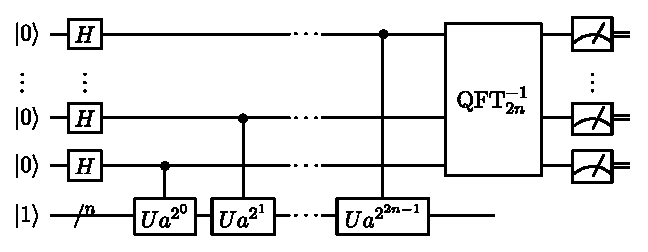
\includegraphics[width=12cm]{pic/Shor_algorithm.eps}
\caption{Circuit of Shor's algorithm}
\label{ShorAlgorithm}
\end{figure}

\subsection{Complexity}

\section{Harrow–Hassidim–Lloyd algorithm}
Harrow–Hassidim–Lloyd (HHL) algorithm approximately solves linear equation $A x = b$ where $x$ and $b$ are $n$ dimensional vectors and $A$ is a $n \times n$ hermitian matrix of complex numbers. The problem would be solved if we knew the orthonormal eigen-vectors ${v_i}, i=1, 2, ...n$ and the eigen-values ${\lambda_i}$ of $A$ because the eigen-values of $A^{-1}$ are  ${1/\lambda_i}$. By writing vector $b$ in terms of the eigen-vectors $b = {\sum^n}_{i=1} \beta_i v_i$, we can achieve our goal
\begin{equation}
    x = A^{-1} b = \sum^{n}_{i=1} \frac {\beta_i} {\lambda_i} v_i .
\end{equation}

Drawing from the technique used in the Deautsch's and Shor's algorithms, we need to "kick up" the eigen-values to the phases. Let's try
\begin{equation}\label{hhl-1}
    e^{i t A}\keta{b} = {\sum^n}_{i=1} \beta_i e^{i t \lambda_i} \keta{v_i}
\end{equation}
where $t$ is a constant to be determined soon. With the circuit of phase estimation, we then can bring the phases down to the second set of qubits
\begin{equation}\label{hhl-2}
    {\sum^n}_{i=1} \beta_i e^{i t \lambda_i} \keta{v_i} \keta{t\lambda_i}.
\end{equation}
We then apply controlled rotation gate to kick values of the second set of qubits to the $\theta$ of a third set of qubits, which contains only one, and have
\begin{equation}\label{hhl-3}
    \sum_{i=1}^n \beta_i e^{i t \lambda_i} \keta{v_i} \keta{t\lambda_i} \keta{cos\theta_i=\frac 1 {t\lambda_i}}.
\end{equation}

Here
\begin{equation}
    \keta{cos\theta_i=\frac 1 {t\lambda_i}} = \frac 1 {t\lambda_i} \keta{0} + sin{\theta_i} \keta{1}.
\end{equation}
If measuring the third set of qubits results in 0, the first and second sets of qubits collaps to
\begin{equation}
    \sum_{i=1}^n \beta_i e^{i t \lambda_i} \keta{v_i} \keta{t\lambda_i} \frac 1 {t\lambda_i}.
\end{equation}

\subsection{Circuit diagram}
\begin{figure}[ht]\label{HHL}
\begin{quantikz}%[slice all, slice style={shorten <=8mm}, slice label style = {yshift=-38mm} ]
    \lstick{\ket{0}} & \qwbundle{1} & \qw               & \qw       & \qw       & \gate{RY}  & \meter{} &\cw \rstick{take result 0} \\
    \lstick{\ket{0}} & \qwbundle{n} &\gate{H^{\otimes n}} &\ctrl{1}     & \gate{IQFT} & \ctrl{-1} & \qw &\gate{QFT} &\ctrl{1}       &\qw  \\
    \lstick{\ket{b}} & \qwbundle{n} & \qw               & \gate{e^{itA}} & \qw       &\qw       &\qw    &\qw       &\gate{e^{-itA}} & \qw \rstick{{\ket{x}}}
\end{quantikz}

\caption{HHL algorithm}
\end{figure}

\subsection{Complexity}

\section{Phase estimate and quantum Fourier transform}

\chapter{Search algorithms}
\section{Grover's algorithm}
Like the Deutsch's algorithm, the Grover's algorithm also assumes a blackbox function $f(x)$ whose variable $x$ is a $n$-bit binary variable while its result is almost always 1 except at a few unknown points $x=x_w$. We assume $f(x_w)=-1$ at these exceptions. The goal of the algorithm is to find the $x_w$. Lov Grover proposed in 1996 that quantum computer can solve it faster than conventional computers.

To illustrate the algorithm, assume there is one and only one $x_w$ which is the search solution. Let's note $x_w$ in binary as $w_{n-1}...w_i...w_1 w_0$ where $w_i = 0 or 1$,
and $\Vec{w} = (0, 0, ..., 1 at i=w, ..., 0)^T$ as a $2^n-1$ dimensional vector.

Using conventional computers, the naive algorithm is to feed the $2^n -1$ possible numbers of $x_w$ one at a time to $f$ to test whether the result equals $-1$. It is a brute force algorithm. The worst case is that we have to do $2^n-1$ evaluations of $f(x)$ to find out $x_w$.

The desired best case is to explore all the possible $x_w$ at the same time. We naturally choose $\vec{S} = \frac 1 {\sqrt{2^n}} (1, 1, ...1)^T$, which is the sum of all the basis of the qubits, to feed the oracle function $f$.

We know, $\vec{S} = \vec{S} - \frac 1 {\sqrt{2^n}} \vec{w}) + \frac 1  {\sqrt{2^n}} \vec{w}$. Apparently, $\vec{S_1}  = \vec{S} - \frac 1 {\sqrt{2^n}} \vec{w}$ is a vector orthogonal to $\vec{w}$, and applying the $F$ gate to it does not change its phase. Therefore, $F(\vec{S}) = F(\vec{S_1}) + F(\frac 1  {\sqrt{2^n}} \vec{w})  = \vec{S_1} - \frac 1 {\sqrt{2^n}} \vec{w}$. We see that 
\begin{itemize}
    \item applying the $F$ gate turns vector $\vec{S}$ toward $-\vec{w}$
    \item applying the $F$ gate to $\vec{S_1}$ makes no change.
\end{itemize}
Therefore, can we apply $F$ gate $2^n$ times and turn $\vec{S}$ completely to $-\vec{w}$? But applying $F$ gate once more will change the phase of the $\vec{w}$ vector back. We need to change the sign of vector $\vec{w}$ first while preserving its angle with $\vec{S}$ before applying $F$ gate again. This can be accomplished by apply gate $U_S = 2 \vec{S}X\vec{S} -I$, which flip $\vec{w}$ around the vector $\vec{S}$. However, when implementing this flip, we need to rotate $vec{S}$ to the $\vec{0}$, do the flip, and rotate the frame back to $\vec{S}$.

\begin{figure}[h]\label{Grover}

\caption{Applying F gate}
\end{figure}

\subsection{Complexity}

\section{Simon's algorithm}
The Simon's algorithm assumes a blackbox oracle function $f(x)$ whose variable $x$ is a $n$-bit binary variable. Its results are $m$-bit values that are periodic, but the period $t$ is unknown -- $f(x+t)=(fx)$ for all $x$. How do we find the period $t$? Of course, we are tempted to play the trick again of feeding $\vec{S} = \frac 1 {\sqrt{2^n}} (1, 1, ...1)^T$ to the oracle function $f$. We have
$f(\vec{S}) = \frac 1  {\sqrt{2^n}} \sum_x f(x)$.

\subsection{Circuit diagram}
\begin{figure}[h]
\begin{quantikz}%[slice all, slice style={shorten <=8mm}, slice label style = {yshift=-38mm} ]
    & & &\lstick{Alice' 2nd bit}  & \cwbend{2} \\
    & & \lstick{1st bit}  & \cwbend{1} \\
    \lstick{\ket{0}} & \gate{H} &\ctrl{1} & \gate{Z} & \gate{X} &\ctrl{1} & \gate{H} & \meter{} &\cw \rstick{Bob's 1st bit} \\
    \lstick{\ket{0}} & \qw      & \targ{} \slice[style={shorten <=12mm}, label style={yshift=-38mm}]{BS1} & \qw \slice[style={shorten <=12mm}, label style={yshift=-38mm}]{BS2} & \qw \slice[style={shorten <=12mm}, label style={yshift=-38mm}]{BS3} & \targ{} & \qw & \meter{} & \cw \rstick{Bob's 2nd bit}
\end{quantikz}
\caption{Simon's algorithm}
\label{Simon}
\end{figure}

\subsection{Complexity}
Using a conventional computer, finding the period takes $2^{n/2}$ operations.

\chapter*{Appendix: Quantum Devices}\label{A-qubit}
\section{Types of waves}
Communication requires waves to propagate from one place to a remote place. Quantum computer qubits require stationary waves. By propagation characteristic, we can differentiate waves into propagating waves, standing waves and trapped waves.

Radio-frequency (RF) electromagnetic waves are used for mobile communications including Wi-Fi. They can spread everywhere unless blocked or confined by reflective matters. Light waves -- electromagnetic waves with wavelength ranging from sub-micron to a few microns -- are used for optical communications. They can be channeled by optical waveguides such as optical fibers to explore different paths. They are confined in two dimensions -- the lateral dimensions -- but propagate in axial dimension along the the waveguides or fibers. Propagating waves are not ideal for building qubits for quantum computing. However, there have been clever designs that construct quantum computing circuits entirely using integrated optical waveguides.

If an electromagnetic wave is confined in three dimensions, such as in a microwave oven, the wave cannot propagate anywhere other than being reflected back and forth within the confinement. And only standing waves of specific frequencies can exist. The allowed frequencies are discrete. Standing waves are good for storing information. Superconductor qubits are constructed using standing waves of electrons, as described below. Standing waves may be best visualized and understood through the vibration of a guitar string. When a string is plucked, the propagation of the vibrations is stopped and reflected by the two fixed ends. Only the waves whose phases coincide after a complete round trip of reflection survive, while the other waves cancel each other out and are suppressed.

Another type of waves, which we may call trapped waves, is not confined by anything with boundaries but is instead trapped by forces extending to infinity. Electrons in an atom are trapped waves due to the electric force of the nucleus' positive charges. The waves extend to infinity but are concentrated within a nanometer around the nucleus. Trapped waves are also good for storing information. Trapped-ion and neutral-atom qubits are built by trapped electron waves.

\section{Devices using polarization modulation}
Polarization is the vibration direction of a wave. The polarization of an electromagnetic wave is perpendicular to its direction of propagation. An electron wave's spin may be considered its polarization and is measurable by applying a magnetic field. The angle of polarization $\theta$ can be used to represent information in addition to the wave's phase $\phi$. Many textbooks use electron spin qubits as examples. However, such type of qubits has not been adopted by practical experiments or products until recently\cite{nanotube} because of the difficulty of building spin-manipulating devices.

Physicists have studied polarization of lights for hundreds of years. Engineers have developed all sorts of polarization-manipulating devices. Combination of polarization and phase modulation has been widely used in communication. The dominating modulation for free-space communication and optical fiber communication is dual polarization quadrature phase shift keying (DP-QPSK). Free space communication is mostly used for satellite-satellite communication. There is no substance in space to degrade the power of light waves. Free space communication can also be used for ship-ship and building-building communication on earth if the distance is not too far. Optical fiber communication is the fastest and cheapest choice for any wired communication of distance 100 meters or longer. The dominant modulation for long-distance optical fiber communication is also DP-QPSK.

Qubits for optical quantum communication naturally use the combination of polarization and phase modulation. Optical qubits have also been demonstrated in laboratories for quantum computing. Gates require manipulating wave polarization. They use optically transparent birefringent materials that have different speeds for lights of different polarization. Placing such a material in a light generator e.g. a laser, generation of light in one polarization direction is favored while the others are suppressed. A half-wave plate made from such a crystal can change the polarization angle of a light to any direction. Fig. \ref{Polarization-splitter} is a type of prism that can split the horizontal and vertical polarization components of a light that has off-angle polarization.

Fig. \ref{Demodulator-DP2} shows the functional diagram of a measurement gate. In communication term, it may be called a demodulator. The input wave from an output qubit is split into two perpendicular polarizing waves. Each wave is further split into two waves with a 90-degree phase difference. A single-photon detector is placed at the end of each wave. Because there is only one quantum of energy in the wave, only one electron in one of the detectors resonates with the wave and registers an electric current. From this detector, we can deduce the modulation point as shown in Fig. \ref{Demodulator-DP2}.

\begin{figure}[h]
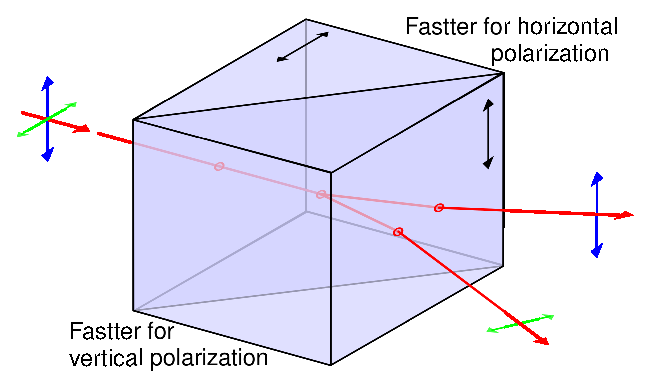
\includegraphics[width=10cm]{pic/polarization-prism.eps}
\caption{Polarization $cos{\theta} \keta{0} + e^{i \phi} sin{\theta} \keta{1}$}
\label{Polarization-splitter}
\end{figure}

\begin{figure}\label{Demodulator-DP2}
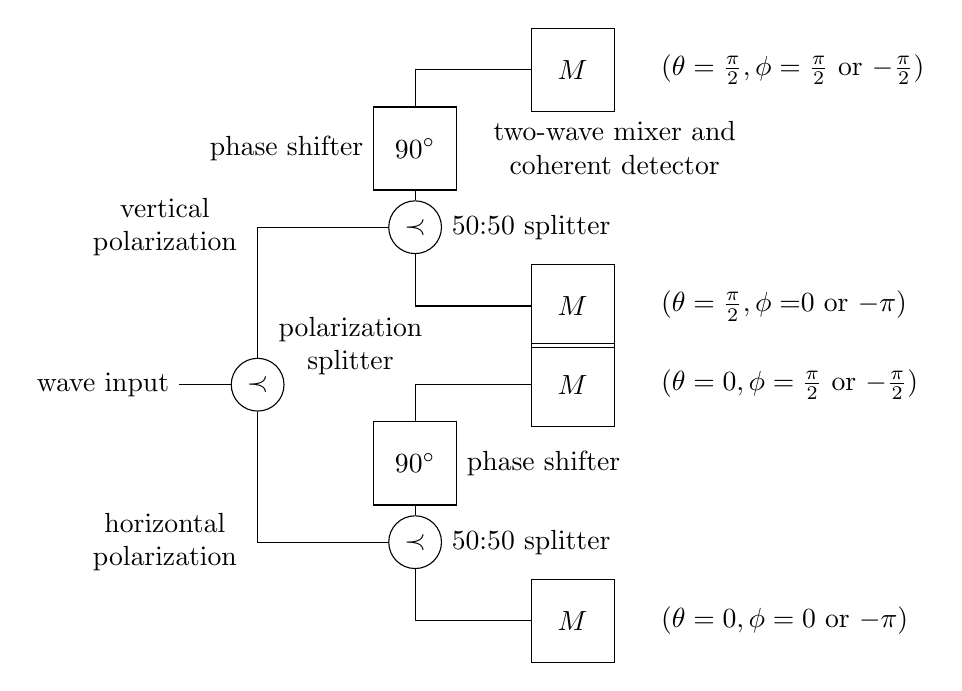
\begin{tikzpicture}[scale=1]
    \path
    (-3,0) node[anchor=east] (input) {wave input}
    (-2,0) node[circle, draw=black] (split) {$\prec$}
%    (-2,1) node[Gate] (theta90) {$90^\circ$}
    (0,2) node[circle, draw=black] (tsp) {$\prec$}
    (0,-2) node[circle, draw=black] (bsp) {$\prec$}
    (0,3) node[Gate] (tphi90) {$90^\circ$}
    (0,-1) node[Gate] (bphi90) {$90^\circ$}
    (2,4) node[Gate] (td1) {$M$}
    (2,1) node[Gate] (td2) {$M$}
    (2,0) node[Gate] (bd1) {$M$}
    (2,-3) node[Gate] (bd2) {$M$};
     
    \path (3,4) node[anchor=west] (bit11) {$(\theta=\frac \pi 2, \phi=\frac \pi 2$ or $-\frac \pi 2)$}
    (3,1) node [anchor=west] (bit10) {$(\theta=\frac \pi 2, \phi=$0 or $-\pi)$}
    (3,0) node [anchor=west] (bit01) {$(\theta=0, \phi=\frac \pi 2$ or $-\frac \pi 2)$}
    (3,-3) node [anchor=west] (bit00) {$(\theta=0, \phi=0$ or $-\pi)$}
    (-2,2) node [text width=60, align=center, anchor=east] (V) {vertical polarization}
    (-2,-2) node [text width=60, align=center, anchor=east] (H) {horizontal polarization};

    \draw (input) -- (split) |- (tsp) -- (tphi90) |- (td1);
    \draw (split) |- (bsp) -- (bphi90) |- (bd1);
    \draw (tsp) |- (td2);
    \draw (bsp) |- (bd2);
    \draw (split) node[text width=60, align=center, anchor=south west] {polarization splitter};
    \draw (tsp.east) node[anchor=west] {50:50 splitter};
    \draw (bsp.east) node[anchor=west] {50:50 splitter};
    \draw (tphi90.west) node[anchor=east] {phase shifter};
    \draw (bphi90.east) node[anchor=west] {phase shifter};
    \draw (td1.south east) node[text width=90, align=center, anchor=north] {two-wave mixer and coherent detector};
\end{tikzpicture}
    \caption{Polarization qubit demodulator}
\end{figure}

\section{Devices using optical waveguides}
Waveguides confine waves in two dimensions and allowing them to propagate in once dimension. Optical fibers are the mostly deployed. A couple of decades ago, radio-frequency cables for broadcasting TV signals were mostly deployed.
Another type of qubits uses lights confined in optical waveguides. Optical fiber is a type of waveguide. We use the optical wave in the waveguide on the left in Fig. \ref{Fiber} to encode the binary number 0 and label it $\keta{0}$. We use the one in waveguide on the right to encode 1 and label it $\keta{1}$. The two waves have the same frequency and amplitude. They don't overlap and are of course orthogonal to each other. If we bring the two waveguides together to overlap (using an optical coupler), we get a superposition wave that is a sum of both waves. If the sum has $cos\theta$ amount in amplitude from $\keta{0}$ wave contributes and $sin\theta_p$ amount in amplitude from the $\keta{1}$ wave, we can use the value $\theta_p$ to characterize the superposition wave.

\begin{figure}[h]\label{Fiber}
%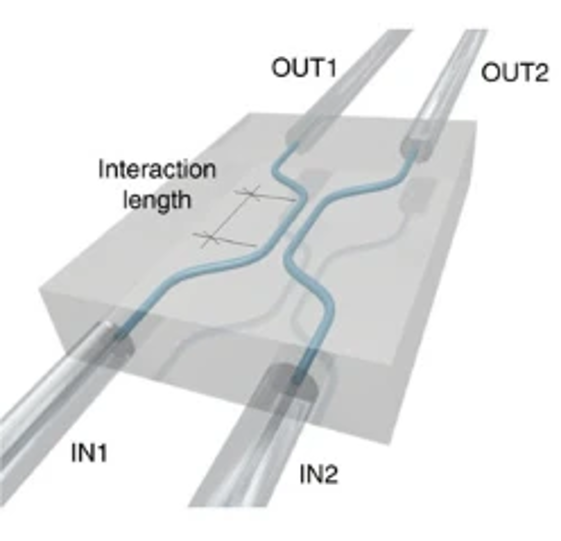
\includegraphics[width=6cm]{pic/wguideQubit.png}
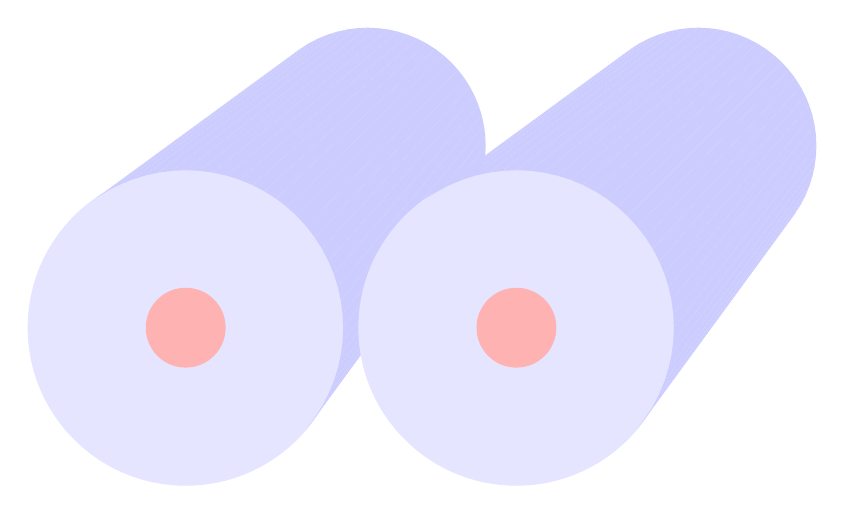
\begin{tikzpicture}[scale=0.5]
    \def\R{4} % Outer radius
    \def\Rb{3} % Outer radius
    \def\r{1} % Inner radius
    \def\L{6} % Half Length of the tube
    \def\S{4.2} % half Shift distance between tubes/fibers
    \def\I{5} % increment

    % Left tube
    \draw[blue!10,fill] (-\S,0,\L) circle (\R);   
    \draw[red!30,fill] (-\S,0,\L) circle (\r);    
    %\draw[decorate,decoration=zigzag] (-\S,0,-\L) circle (\Rb);
    \foreach \t in {-40,-35,...,123} {
        \fill[blue!20] ({\R*cos(\t+\I)-\S}, {\R*sin(\t+\I)}, \L) -- ({\R*cos(\t)-\S}, {\R*sin(\t)}, \L) 
        -- ({\Rb*cos(\t)-\S}, {\Rb*sin(\t)}, -\L) -- ({\Rb*cos(\t+\I)-\S}, {\Rb*sin(\t+\I)}, -\L) -- cycle;
    }

    % Right tube    
    \draw[blue!10,fill] (\S,0,\L) circle (\R);   
    \draw[red!30,fill] (\S,0,\L) circle (\r);    
    %\draw[black!10] (\S,0,-\L) circle (\Rb);
    \foreach \t in {-40,-35,...,123} {
        \fill[blue!20] ({\R*cos(\t+\I)+\S}, {\R*sin(\t+\I)}, \L) -- ({\R*cos(\t)+\S}, {\R*sin(\t)}, \L) 
        -- ({\Rb*cos(\t)+\S}, {\Rb*sin(\t)}, -\L) -- ({\Rb*cos(\t+\I)+\S}, {\Rb*sin(\t+\I)}, -\L) -- cycle;
    }
\end{tikzpicture}
\caption{A waveguide qubit comprised by two single-mode optical fibers $cos{\theta} \keta{0} + e^{i \phi} sin{\theta} \keta{1}$}
\end{figure}

The Xanadu.ai M-8 quantum computing chip assembles waveguide qubits and processing gates in an integrated waveguide circuit. We see it very much resembles a maze. The optical waveguides are the paths that light waves traverse. Its couplers and splitters resemble the junctions of maze. A coupler merge two light paths into one, and a splitter split one into two. The chip has 8 entrances and 8 exits and can build $8^8$ possible paths.

%\backmatter

\addcontentsline{toc}{chapter}{Bibliography}
\chapter*{Bibliography}
\bibliographystyle{unsrt}
   \bibliography{qcc}

\addcontentsline{toc}{chapter}{Index}
\printindex
\end{document}